% Informe de la Tarea 2 de Hidrología (202602).
% Compilar desde esta carpeta:  pdflatex informe.tex  (dos veces)
% Las cifras se leen de los archivos generados por los scripts:
%   productos/punto1/cifras_punto1.tex  <- codigo/punto1/cifras_punto1.py
%   productos/punto2/final/cifras_punto2.tex  <- codigo/punto2/analisis_final_punto2.py
\documentclass[12pt,a4paper]{article}
\usepackage[utf8]{inputenc}
\usepackage[T1]{fontenc}
\usepackage[spanish,es-nodecimaldot,es-noshorthands,es-tabla]{babel}
\usepackage{amsmath}
\usepackage{newtxtext,newtxmath}
\usepackage{graphicx}
\usepackage{booktabs}
\usepackage[margin=2.54cm]{geometry}
\usepackage{setspace}
\usepackage{caption}
\usepackage{float}
\usepackage{xcolor}
\usepackage{tikz}
\usetikzlibrary{positioning,arrows.meta}
\usepackage[hidelinks]{hyperref}

% Generado por codigo/punto1/cifras_punto1.py. No editar a mano.
\newcommand{\EToAnual}{1179}
\newcommand{\EToMesMin}{86}
\newcommand{\EToMesMax}{110}
\newcommand{\DifPromMax}{0{,}30}
\newcommand{\DifPuntoMax}{1{,}58}
\newcommand{\DzMin}{$-$806}
\newcommand{\DzMax}{394}
\newcommand{\DzPond}{18}
\newcommand{\CobEra}{90{,}1}
\newcommand{\PmQfis}{605}
\newcommand{\EToFis}{1182}
\newcommand{\TCr}{0{,}90}
\newcommand{\TCsesgo}{1{,}4}
\newcommand{\TCmae}{4{,}0}
\newcommand{\PIr}{0{,}70}
\newcommand{\PIsesgo}{$-$1{,}0}
\newcommand{\PImae}{8{,}0}
\newcommand{\NOr}{0{,}81}
\newcommand{\NOsesgo}{4{,}7}
\newcommand{\NOmae}{11{,}1}
\newcommand{\MAEThorn}{38{,}7}
\newcommand{\SesgoThorn}{$-$39}
\newcommand{\RThorn}{0{,}57}
\newcommand{\MAEHarg}{6{,}1}
\newcommand{\SesgoHarg}{$-$6}
\newcommand{\RHarg}{0{,}92}
\newcommand{\MAEPT}{20{,}2}
\newcommand{\SesgoPT}{21}
\newcommand{\RPT}{0{,}96}
\newcommand{\MAEMeyer}{58{,}6}
\newcommand{\SesgoMeyer}{$-$60}
\newcommand{\RMeyer}{0{,}56}
\newcommand{\MAEMakk}{5{,}0}
\newcommand{\SesgoMakk}{5}
\newcommand{\RMakk}{0{,}98}
\newcommand{\MAERohw}{53{,}9}
\newcommand{\SesgoRohw}{$-$55}
\newcommand{\RRohw}{0{,}54}
\newcommand{\FracRadMin}{83}
\newcommand{\FracRadMax}{92}
\newcommand{\AlfaMin}{1{,}00}
\newcommand{\AlfaMax}{1{,}09}
\newcommand{\VPDMin}{0{,}36}
\newcommand{\VPDMax}{0{,}68}
\newcommand{\SensRs}{$-$85}
\newcommand{\SensPctRs}{$-$7{,}2}
\newcommand{\SensTunoEa}{42}
\newcommand{\SensPctTunoEa}{3{,}6}
\newcommand{\SensTunoHR}{30}
\newcommand{\SensPctTunoHR}{2{,}5}
\newcommand{\SensTdosEa}{83}
\newcommand{\SensPctTdosEa}{7{,}0}
\newcommand{\SensTdosHR}{60}
\newcommand{\SensPctTdosHR}{5{,}1}
\newcommand{\SensEa}{$-$20}
\newcommand{\SensPctEa}{$-$1{,}7}
\newcommand{\SensUdos}{4}
\newcommand{\SensPctUdos}{0{,}3}
\newcommand{\SensThornTuno}{4{,}5}
\newcommand{\ETgleam}{740}
\newcommand{\ETmod}{796}
\newcommand{\ETbalL}{603}
\newcommand{\ETbalI}{73}
\newcommand{\SobreGleam}{23}
\newcommand{\SobreMod}{32}
\newcommand{\PL}{1104}
\newcommand{\Qmed}{501}
\newcommand{\DifPLPI}{530}
\newcommand{\SigmaP}{175}
\newcommand{\SigmaQ}{38}
\newcommand{\SigmaET}{180}
\newcommand{\SigmaETpct}{30}
\newcommand{\RnLambda}{1743}
\newcommand{\FEbal}{0{,}35}
\newcommand{\EToHumMin}{0{,}72}
\newcommand{\EToHumMax}{0{,}89}
\newcommand{\EToSecMin}{0{,}43}
\newcommand{\EToSecMax}{0{,}62}
\newcommand{\CorrFEg}{0{,}92}
\newcommand{\CorrFEm}{0{,}91}
\newcommand{\KnotG}{0{,}31}
\newcommand{\KnotM}{0{,}36}
\newcommand{\PhiAr}{1{,}08}
\newcommand{\EIg}{0{,}67}
\newcommand{\EIm}{0{,}72}
\newcommand{\OmG}{2{,}28}
\newcommand{\OmM}{2{,}59}
\newcommand{\BudyEI}{0{,}64}
\newcommand{\DistG}{0{,}03}
\newcommand{\DistM}{0{,}08}
\newcommand{\ElasG}{1{,}95}
\newcommand{\ElasM}{2{,}19}
\newcommand{\PhiI}{2{,}08}
\newcommand{\EToSeco}{1211}
\newcommand{\EToHumedo}{1173}
\newcommand{\ETSecoG}{707}
\newcommand{\ETHumG}{776}
\newcommand{\CorrPETo}{$-$0{,}75}
\newcommand{\TendETo}{1{,}14}
\newcommand{\pETo}{0{,}0026}
\newcommand{\TendTh}{0{,}57}
\newcommand{\pTh}{0{,}0005}
\newcommand{\TendT}{0{,}18}
\newcommand{\AtrT}{0{,}76}
\newcommand{\AtrEa}{$-$0{,}13}
\newcommand{\AtrUdos}{0{,}01}
\newcommand{\AtrRs}{0{,}57}
\newcommand{\AtrSuma}{1{,}21}
\newcommand{\AtrRes}{$-$0{,}05}
\newcommand{\EToBajo}{1307}
\newcommand{\EToAlto}{1083}
\newcommand{\GlBajo}{801}
\newcommand{\GlAlto}{604}
\newcommand{\ModBajo}{575}
\newcommand{\ModAlto}{813}
\newcommand{\ModMax}{889}
\newcommand{\ModMaxBanda}{2750-3250 m}

% Generado por codigo/punto2/analisis_final_punto2.py. No editar a mano.
\newcommand{\NAnios}{20}
\newcommand{\AreaMicro}{0{,}123}
\newcommand{\LongCauce}{382{,}7}
\newcommand{\PendCauce}{0{,}125}
\newcommand{\Cpre}{0{,}332}
\newcommand{\Cpremenos}{0{,}266}
\newcommand{\Cpremas}{0{,}399}
\newcommand{\Curb}{0{,}60}
\newcommand{\tcKirpich}{4{,}2}
\newcommand{\tcKerby}{21{,}5}
\newcommand{\tcSCS}{12{,}5}
\newcommand{\tcUrb}{7{,}6}
\newcommand{\Tdis}{25}
\newcommand{\Vida}{30}
\newcommand{\RiesgoNom}{70{,}6}
\newcommand{\RiesgoAcept}{75}
\newcommand{\Treq}{22{,}1}
\newcommand{\Idis}{129{,}8}
\newcommand{\Qp}{1{,}476}
\newcommand{\Dcalc}{0{,}83}
\newcommand{\Dcom}{0{,}90}
\newcommand{\Qcap}{1{,}81}
\newcommand{\FS}{1{,}23}
\newcommand{\Drec}{1{,}05}
\newcommand{\QcapRec}{2{,}73}
\newcommand{\FSrec}{1{,}85}
\newcommand{\PeffRec}{1{,}05}
\newcommand{\TeffRec}{95}
\newcommand{\RiesgoEffRec}{27{,}2}
\newcommand{\Peff}{4{,}97}
\newcommand{\Teff}{20}
\newcommand{\RiesgoEff}{78{,}3}
\newcommand{\ProbQLQc}{30{,}8}
\newcommand{\QLlo}{0{,}92}
\newcommand{\QLhi}{2{,}69}
\newcommand{\Dlo}{0{,}70}
\newcommand{\Dhi}{1{,}04}
\newcommand{\NMC}{5000}
\newcommand{\NBoot}{500}
\newcommand{\WeissDiez}{1{,}143}
\newcommand{\WeissHora}{1{,}021}
\newcommand{\QdiezTcien}{32{,}7}
\newcommand{\QhoraTcien}{69{,}7}
\newcommand{\KosHoraTcien}{45{,}9}
\newcommand{\RazonHoraTcien}{1{,}52}
\newcommand{\KosUCHoraTcien}{26}
\newcommand{\SinHoraTcien}{55{,}5}
\newcommand{\RazonDiezTveinte}{1{,}12}
\newcommand{\IDFtheta}{0{,}120}
\newcommand{\IDFeta}{0{,}828}
\newcommand{\IDFrmse}{1{,}8}
\newcommand{\IDFerr}{11{,}1}
\newcommand{\IDFrdos}{0{,}999}
\newcommand{\Qpre}{1{,}476}
\newcommand{\DOrif}{0{,}701}
\newcommand{\Cd}{0{,}61}
\newcommand{\Hutil}{2{,}0}
\newcommand{\VolCrit}{1350}
\newcommand{\EscCrit}{bloques alternos + tiempo-area, pico al centro}
\newcommand{\LadoTanque}{26{,}0}
\newcommand{\VolUtil}{1352}
\newcommand{\VolTrap}{993}
\newcommand{\TrapCrit}{d=15 min}
\newcommand{\VolInicio}{979}
\newcommand{\VolCentro}{1350}
\newcommand{\VolFinal}{1288}
\newcommand{\QsalMax}{1{,}475}
\newcommand{\TeventoTrece}{196}
\newcommand{\TeventoVeintiuno}{28{,}1}
\newcommand{\TeventoVeintiunoLo}{8{,}4}
\newcommand{\TeventoVeintiunoHi}{3265}
\newcommand{\AnchoTcien}{57}
\newcommand{\CompletMin}{98{,}54}

% Generado por codigo/punto2/contraste_evento_2013.py
\newcommand{\EvRadarEst}{33{,}8}
\newcommand{\EvRadarTresEst}{45{,}8}
\newcommand{\EvRadarMaxVent}{67{,}8}
\newcommand{\EvAreaCuarenta}{168}
\newcommand{\EvBuhler}{59{,}5}
\newcommand{\EvNeubronn}{34{,}6}
\newcommand{\EvGoggingen}{27{,}7}
\newcommand{\EvAalen}{12{,}9}
\newcommand{\EvHeubach}{11{,}5}
\newcommand{\EvGmundHora}{17{,}1}
\newcommand{\EvEllwHora}{7{,}6}
\newcommand{\EvGmundDia}{22{,}2}
\newcommand{\EvGmundKm}{17}
\newcommand{\EvEllwKm}{18}
\newcommand{\EvBuhlerKm}{9}
\newcommand{\EvRadarBuhler}{33{,}2}
\newcommand{\VecGmundAnios}{23}
\newcommand{\VecEllwAnios}{23}
\newcommand{\VecGmundComp}{98{,}9}
\newcommand{\VecEllwComp}{99{,}5}
\newcommand{\VecGmundQcien}{59{,}7}
\newcommand{\VecEllwQcien}{59{,}3}
\newcommand{\VecPropQcien}{69{,}8}
\newcommand{\VecRhoGmund}{0{,}30}
\newcommand{\VecRhoEllw}{0{,}21}

\graphicspath{{../../productos/punto1/}{../../productos/punto2/final/figuras/}{../../datos/punto2/Abtsgmuend_Untergroeningen/control_2_1/}}

% Citas autor-anio en formato APA 7 (sin biblatex)
\makeatletter
\newcommand{\defref}[3]{\expandafter\def\csname rA@#1\endcsname{#2}\expandafter\def\csname rY@#1\endcsname{#3}}
\newcommand{\parencite}[2][]{(\@tempswafalse\@for\rk:=#2\do{\if@tempswa; \fi\@tempswatrue\csname rA@\rk\endcsname, \csname rY@\rk\endcsname}\ifx\relax#1\relax\else, #1\fi)}
\newcommand{\textcite}[2][]{\csname rA@#2\endcsname\ (\csname rY@#2\endcsname\ifx\relax#1\relax\else, #1\fi)}
\makeatother
\defref{abatzoglou2018}{Abatzoglou et al.}{2018}
\defref{allen1998}{Allen et al.}{1998}
\defref{bouchet1963}{Bouchet}{1963}
\defref{brutsaert1998}{Brutsaert y Parlange}{1998}
\defref{budyko1974}{Budyko}{1974}
\defref{chow1988}{Chow et al.}{1988}
\defref{coles2001}{Coles}{2001}
\defref{dejong2005}{de Jong et al.}{2005}
\defref{dwd2022}{Deutscher Wetterdienst}{2022}
\defref{dwd2026}{Deutscher Wetterdienst}{2026}
\defref{dingman2015}{Dingman}{2015}
\defref{fu1981}{Fu}{1981}
\defref{gringorten1963}{Gringorten}{1963}
\defref{hosking1997}{Hosking y Wallis}{1997}
\defref{hoyos2026}{Hoyos}{2026}
\defref{koutsoyiannis1998}{Koutsoyiannis et al.}{1998}
\defref{debruin1987}{de Bruin}{1987}
\defref{makkink1957}{Makkink}{1957}
\defref{kuiry2021}{Kuiry y Sen}{2021}
\defref{martins2000}{Martins y Stedinger}{2000}
\defref{mcvicar2012}{McVicar et al.}{2012}
\defref{milly2016}{Milly y Dunne}{2016}
\defref{miralles2011}{Miralles et al.}{2011}
\defref{mu2011}{Mu et al.}{2011}
\defref{munozsabater2021}{Muñoz-Sabater et al.}{2021}
\defref{nrcs2010}{Natural Resources Conservation Service}{2010}
\defref{pastorello2020}{Pastorello et al.}{2020}
\defref{roderick2002}{Roderick y Farquhar}{2002}
\defref{sankarasubramanian2001}{Sankarasubramanian et al.}{2001}
\defref{shaw2010}{Shaw et al.}{2010}
\defref{svensson2010}{Svensson y Jones}{2010}
\defref{usgs2013}{U.S. Geological Survey}{2013}
\defref{weiss1964}{Weiss}{1964}
\defref{westra2014}{Westra et al.}{2014}
\defref{zanaga2022}{Zanaga et al.}{2022}

% Datos que debe completar el grupo
\newcommand{\Grupo}{G\textcolor{red}{XX}}
\newcommand{\PENDIENTE}[1]{\textcolor{red}{[PENDIENTE DEL GRUPO: #1]}}

% Formato APA 7: titulo de tabla/figura en negrita arriba y titulo en cursiva debajo
\captionsetup{labelfont=bf,textfont=it,labelsep=newline,justification=raggedright,singlelinecheck=false,position=top,skip=4pt}
\captionsetup[figure]{name=Figura}
\captionsetup[table]{name=Tabla}
\newcommand{\nota}[1]{\par\vspace{2pt}{\footnotesize\raggedright\textit{Nota.} #1\par}}
\setlength{\parindent}{1.27cm}
\onehalfspacing
\renewcommand{\thesection}{\arabic{section}}
\setcounter{secnumdepth}{3}

\begin{document}
\sloppy

% ------------------------------------------------------------------ portada
\begin{titlepage}
\centering
\vspace*{3cm}
{\bfseries Tarea 2. Evapotranspiración y diseño hidrológico}\par
\vspace{1.2cm}
Andrés Francisco Idrobo Hidrobo, Enmaly Aleli Manturano Grajeda y Jeyson Cristian Javier Irpanoca\par
\vspace{0.6cm}
Grupo \Grupo\par
\vspace{0.6cm}
Facultad de Minas, Universidad Nacional de Colombia, Sede Medellín\par
\vspace{0.6cm}
Hidrología, semestre 202602\par
Profesor: Carlos David Hoyos\par
\vspace{0.6cm}
24 de noviembre de 2026
\end{titlepage}

\tableofcontents
\newpage

% ================================================================== 1
\section{Introducción}

En la Tarea 1 describimos cuándo llega el agua a la cuenca PE\_200907 (río Chancay--Lambayeque en la estación Racarumi, norte del Perú, 2363 km$^2$) y cuándo sale por el río. Entre esas dos series queda el término que no se midió: el agua que la cuenca devuelve a la atmósfera. Esta tarea lo estima (punto 1) y, en un sitio distinto con lluvia subdiaria, dimensiona dos obras de drenaje con su incertidumbre (punto 2).

\textbf{Cuenca del punto 1.} La cuenca drena la vertiente occidental de los Andes entre 264 y 4084 m de altitud. Su régimen es tropical estacional: la temporada húmeda va de enero a abril y la seca de junio a septiembre. Con PISCOp v2.1 la precipitación media es \PL\ mm/año y la escorrentía \Qmed\ mm/año. En el promedio de largo plazo la diferencia, unos 600 mm/año, es la mayor salida del balance. La cuenca tiene una bocatoma (Racarumi) y recibe trasvases desde las cuencas del Chotano y el Conchano, documentados en los planes regionales consultados (anexo \texttt{anexos/punto1/1\_3\_regimen\_evaporativo/fuentes\_documentales/}).

\textbf{Sitio del punto 2.} La cuenca del punto 1 no tiene una serie de lluvia subdiaria suficiente: las estaciones peruanas revisadas solo tenían acumulados diarios o tramos horarios cortos. Siguiendo los criterios del enunciado (longitud del registro y luego resolución), se escogió la estación 00020 del Servicio Meteorológico Alemán (DWD), Abtsgmünd--Untergröningen (Baden-Wurtemberg; 48,92° N, 9,91° E; 432 m), con lluvia cada 10 minutos entre 2005 y 2025 \parencite{dwd2026}. El clima es templado oceánico y las lluvias intensas son tormentas convectivas de verano.

\textbf{Preguntas e hipótesis.}
\begin{enumerate}
\item ¿Cuál es la demanda evaporativa de la cuenca y qué la controla? Hipótesis: en una cuenca tropical de montaña con poco viento, la demanda está dominada por la radiación; los métodos solo térmicos la representan mal porque la temperatura casi no tiene ciclo anual.
\item ¿Cuánta agua devuelve la cuenca y con qué incertidumbre? Hipótesis: la incertidumbre de la precipitación domina la del balance $P-Q$.
\item ¿En qué meses manda la energía y en cuáles el agua? Hipótesis: la evapotranspiración está limitada por energía en la temporada húmeda y por agua en la seca, y el promedio multianual se ubica en la transición del espacio de Budyko.
\item ¿Qué lluvia debe soportar una alcantarilla, con qué riesgo real y con qué incertidumbre en su tamaño? Hipótesis: la incertidumbre de la cola de la distribución de extremos, con solo \NAnios\ años, domina sobre la del coeficiente de escorrentía y el tiempo de concentración.
\end{enumerate}

% ================================================================== 2
\section{Metodología}

\subsection{Punto 1: datos y procedimientos}

\textbf{Series de la Tarea 1.} Se reutilizaron las series mensuales de precipitación (PISCOp v2.1, en adelante $P_L$; IMERG Final V07, $P_I$), caudal observado y temperatura (PISCOt v1.2) de CAMELS-PE, con los criterios de faltantes de la Tarea 1: meses de caudal con menos de 90\,\% de días válidos quedan sin dato y no se imputó ningún valor. El año hidrológico va de septiembre a agosto, que empieza en la época de menor almacenamiento.

\textbf{ETo FAO-56 (1.1.a).} Se calculó la ETo diaria con la ecuación 6 de \textcite{allen1998} a partir de series horarias de ERA5-Land \parencite{munozsabater2021} en las celdas que cubren la cuenca, y se agregó a meses al final. $T_{\max}$ y $T_{\min}$ salen de las 24 horas de cada día; $e_s=\tfrac12[e(T_{\max})+e(T_{\min})]$; $e_a=e(T_d)$; la magnitud del viento se calculó hora a hora antes de promediar y se redujo de 10 a 2 m con la ecuación 47; $R_n$ es la del pasto de referencia (albedo 0,23, ecuación 39 para $R_{nl}$); $G\approx0$ en el cálculo diario; la presión corresponde a la elevación media de cada celda. Cada celda se procesó por separado y se ponderó con los pesos de intersección de la Tarea 1. Se obtuvieron 20 de las 33 celdas, que representan el \CobEra\,\% del peso espacial de la cuenca; las 13 celdas restantes no se pudieron descargar porque el servicio CDS rechazó la autenticación de la cuenta (error 401). Los pesos se renormalizaron sobre las celdas disponibles; esta es una limitación declarada. También se calculó la ETo con medias mensuales de las variables, con $G_i=0{,}07(T_{i+1}-T_{i-1})$, para medir el error por promediar antes de una ecuación no lineal.

\textbf{Pruebas de la referencia (1.1.b).} (1) La estación GHCNh de Chiclayo (PEI0000SPHI), fuera de la cuenca y en la costa, con $R_s$ estimada por la ecuación 50 de FAO-56 ($k_{Rs}=0{,}16$ y $0{,}19$), comparada con ERA5-Land en la misma celda para separar el error del reanálisis del error del método. (2) Dos productos independientes de demanda: la PET Penman-Monteith de PISCOeo\_pm incluida en CAMELS-PE y la ETo de TerraClimate \parencite{abatzoglou2018}. (3) La restricción física de que la ETo multianual supere a $P-Q$.

\textbf{Métodos alternativos (1.1.c).} Se calcularon cuatro métodos de la tabla del enunciado, uno por familia: Thornthwaite (temperatura), Hargreaves--Samani (temperatura y $R_a$), Priestley--Taylor con $\alpha=1{,}26$ (radiación) y Meyer (transferencia de masa). Se añadieron dos métodos de principio físico distinto: Makkink, basado en la radiación solar, y Rohwer, de transferencia de masa con viento a 0,6 m. De Makkink se usó la variante de \textcite{debruin1987}, $0{,}65\,\Delta/(\Delta+\gamma)\,R_s/\lambda$ sin constante, que es la que implementa \texttt{pyet} y la que usa el servicio meteorológico de los Países Bajos; como sensibilidad se calculó también la forma original de \textcite{makkink1957}, $0{,}61\,\Delta/(\Delta+\gamma)\,R_s/\lambda-0{,}12$ mm/d \parencite[sec.~7]{hoyos2026}. Las ecuaciones, sus versiones y unidades están en el anexo \texttt{anexos/punto1/1\_1\_c\_metodos\_alternativos/}. Thornthwaite y Hargreaves se verificaron con un cálculo a mano; Priestley--Taylor y Makkink se calcularon con \texttt{pyet} 1.5.0. Siguiendo el árbol de decisión de las notas del curso, el coeficiente 0,0023 de Hargreaves se calibró contra la ETo FAO-56 con el cociente de sumas en 1981--2001 y se validó en 2002--2022 (\texttt{calibrar\_hargreaves\_1\_1d.py}). El ajuste a FAO-56 se midió con sesgo, MAE, RMSE y la amplitud y fase del primer armónico, por mes calendario.

\textbf{Explicación de las diferencias (1.1.d).} FAO-56 se separó en su término radiativo y su término aerodinámico; se calculó $\alpha^*=\mathrm{ETo}/E_{eq}$ con $E_{eq}=\Delta(R_n-G)/[(\Delta+\gamma)\lambda]$. Se perturbaron $T$ (+1 y +2 °C, con $e_a$ constante y con humedad relativa constante), $u_2$ (+10\,\%), $R_s$ ($-10$\,\%) y $e_a$ (+10\,\%), y se recalcularon todos los métodos.

\textbf{Evapotranspiración real (1.2).} Balance $ET=P-Q$ con $P_L$ y $P_I$ en años hidrológicos completos; propagación $\sigma^2_{ET}=\sigma^2_P+\sigma^2_Q$ con $\sigma_P$ igual a la dispersión entre $P_L$ y $P_I$ y una incertidumbre del caudal de $\pm15$\,\% (escenarios de 10 y 20\,\%), a falta de la curva de gasto de Racarumi; techo energético $R_n/\lambda$ con la radiación neta real de ERA5-Land ($SSR+STR$); comparación con GLEAM v4.3a \parencite{miralles2011} y MOD16A2GF v6.1 \parencite{mu2011} en el periodo común (años hidrológicos 2002 y 2004--2023). Se revisó la disponibilidad de torres de covarianza de remolinos en la región \parencite{pastorello2020}.

\textbf{Régimen evaporativo (1.3).} Cocientes mensuales $ET/\mathrm{ETo}$ y $ET/P$ con los dos productos; fracción evaporativa frente a la humedad de la zona de raíces de ERA5-Land (0--100 cm, $0{,}07\,swvl_1+0{,}21\,swvl_2+0{,}72\,swvl_3$); ubicación en el espacio de Budyko con la curva de \textcite{fu1981} ajustada; elasticidad teórica $\varepsilon_P=1+\phi F'(\phi)/(1-F(\phi))$ frente a la empírica con el estimador de mediana de \textcite{sankarasubramanian2001}; comparación de $ET$ y ETo en terciles secos, normales y húmedos. Se usó ETo en lugar de la evapotranspiración potencial de Budyko y se declara así.

\textbf{Cambios en la demanda (1.4).} Mann--Kendall y pendiente de Sen anuales y por mes calendario, con corrección de Benjamini--Hochberg, preblanqueo sin tendencia (TFPW) cuando la autocorrelación de orden 1 fue significativa, errores de Newey--West y 49 escenarios de recorte y exclusión de un año (1981--2022). La atribución usó sensibilidades numéricas $\partial\mathrm{ETo}/\partial x_i$ de la ecuación diaria multiplicadas por la tendencia de cada forzante.

\textbf{Paisaje (1.5).} Se eligió el tema (a), gradiente altitudinal: la cuenca cubre 3800 m de desnivel y la Tarea 1 mostró que la lluvia y la temperatura cambian con la altura. Se definieron ocho bandas de 500 m con el DEM SRTM y se estimaron por banda la ETo FAO-56 (celda a celda) y la ET de GLEAM y MOD16. Se descartaron: nieve y sublimación (no hay glaciares ni nieve estacional en la cuenca), agua libre y riego como tema principal (el embalse Tinajones queda fuera de la cuenca), niebla (no hay datos de nubosidad baja ni de captación) e intercepción y resistencia del dosel (no hay datos de lluvia por evento bajo dosel ni de índice de área foliar procesado).

\subsection{Punto 2: datos y procedimientos}

\textbf{Serie y control de calidad (2.1).} Se unificaron los tres archivos históricos de precipitación de 10 minutos del DWD (variable RWS\_10, mm en los 10 minutos anteriores, hora UTC). Los códigos de faltante ($-999$) se marcaron como ausentes sin imputar. El año hidrológico va de octubre a septiembre, para que la temporada convectiva de verano quede entera dentro de cada año; 2004 se excluyó por incompleto. Un año aporta un máximo válido si tiene al menos 80\,\% de registros y 90\,\% en mayo--septiembre; todos los años superaron el \CompletMin\,\%, por lo que no se descartó ninguno y el criterio no afecta los cuantiles. Se revisaron intervalos de tiempo, códigos de calidad, valores repetidos y acumulados tras vacíos, y se contrastó el máximo de 24 h de cada año con la mayor lluvia diaria de reloj del mismo año (tabla \texttt{control\_ams\_vs\_diaria.csv}). Los máximos anuales se contrastaron con estaciones vecinas del DWD: dos estaciones de 10 minutos con registro largo, Schwäbisch Gmünd-Weiler (06262, a \EvGmundKm\ km) y Ellwangen-Rindelbach (01197, a \EvEllwKm\ km), que cumplen los mismos requisitos de 2.1 (\VecGmundAnios\ y \VecEllwAnios\ años válidos, completitud mínima de \VecGmundComp\ y \VecEllwComp\,\%); seis pluviómetros diarios en un radio de 15 km, y el radar RADOLAN RW del DWD (horario, 1 km). Los datos y su preparación están en \texttt{datos/punto2/vecinas\_2013/} y \texttt{codigo/punto2/descargar\_vecinas\_2013.py}. La microcuenca se delimitó con el DEM SRTM de 1'' \parencite{usgs2013} y la cobertura se obtuvo de ESA WorldCover 2021 v200 \parencite{zanaga2022}.

\textbf{Corrección de Weiss.} Los datos son acumulados en intervalos fijos de reloj de 10 minutos. Aunque los máximos se buscan con ventanas móviles, cada ventana está formada por $n$ intervalos fijos, que es precisamente el caso del factor de \textcite{weiss1964}, $1/(1-1/(8n))$: \WeissDiez\ para 10 minutos y \WeissHora\ para 1 hora. Se aplicó a los máximos anuales antes del ajuste. La versión previa del análisis no lo aplicaba; ese cambio sube los cuantiles de 10 minutos en un 14\,\%.

\textbf{Extremos (2.2).} Máximos anuales con ventanas móviles para 10 y 30 minutos y 1, 3, 6, 12 y 24 horas, con verificación de que la profundidad no disminuye con la duración. Se ajustaron GEV (máxima verosimilitud, L-momentos y máxima verosimilitud generalizada), Gumbel (máxima verosimilitud y L-momentos) y log-Pearson III (momentos en el espacio logarítmico). La bondad de ajuste se evaluó con Kolmogorov--Smirnov, Cramér--von Mises y el coeficiente de correlación de la gráfica de probabilidad (PPCC) con posiciones de Gringorten \parencite{gringorten1963}, que es la recomendada para GEV y Gumbel, y con el diagrama de razones de L-momentos \parencite{hosking1997}. La incertidumbre se estimó con \NBoot\ réplicas bootstrap remuestreando años completos, de modo que se conserva la coherencia entre duraciones. La tendencia se revisó con Mann--Kendall y Sen.

\textbf{Elección de la distribución.} La GEV por máxima verosimilitud dio formas muy pesadas ($\xi$ hasta 0,5) y, en el bootstrap, réplicas degeneradas con cuantiles de 100 años sin sentido físico; es la inestabilidad de la forma con muestras cortas que señala \textcite{coles2001}. Por eso se usó como distribución de diseño la GEV por máxima verosimilitud generalizada (GMLE) de \textcite{martins2000}, que añade una distribución previa Beta(6, 9) para la forma y estabiliza los cuantiles altos sin forzar una cola liviana. La GEV por máxima verosimilitud clásica, Gumbel y log-Pearson III se conservan como sensibilidad.

\textbf{Curvas IDF (2.3).} Se ajustó la forma de \textcite{koutsoyiannis1998}, $i(d,T)=w(T)/(d+\theta)^{\eta}$, con $\theta$ y $\eta$ comunes a todos los periodos de retorno, a los cuantiles de las siete duraciones. Se comparó con KOSTRA-DWD-2020 \parencite{dwd2022} en la celda de la estación, incluida su incertidumbre publicada (UC).

\textbf{Diseño (2.4).} Método racional $Q_p=C\,i(t_c,T)\,A/3{,}6$; $C$ ponderado por área con WorldCover y coeficientes de \textcite[tabla 15.1.1]{chow1988}; $t_c$ con Kirpich, Kerby y el retardo del SCS \parencite{nrcs2010}; diámetro con Manning, $D=[nQ/(0{,}312\,S_0^{1/2})]^{3/8}$, redondeado al diámetro comercial superior. El riesgo efectivo se estimó con \NMC\ simulaciones de Monte Carlo que muestrean una réplica bootstrap de la IDF, $C$ ($\pm20$\,\%), $t_c$ (triangular en escala logarítmica entre Kirpich y Kerby, con moda en el valor de diseño), $n$ de Manning (0,011--0,015) y la pendiente construida ($0{,}010\pm0{,}001$). El tanque se dimensionó con el racional modificado (hidrogramas trapezoidales), el método de bloques alternos con el racional de tiempo-área y tránsito por piscina nivelada con salida por orificio \parencite[cap.~3]{kuiry2021}.

Todo el procesamiento del punto 2 está en \texttt{codigo/punto2/analisis\_final\_punto2.py}; las decisiones de ingeniería se leen de \texttt{codigo/punto2/config\_diseno\_2\_4.json}.

% ================================================================== 3
\section{Resultados y discusión física}

\subsection{Punto 1. La demanda atmosférica}

\textbf{Magnitud y ciclo anual.} La ETo FAO-56 de la cuenca es de unos \EToAnual\ mm/año, con valores mensuales entre \EToMesMin\ y \EToMesMax\ mm. El máximo cae en octubre--noviembre, al final de la temporada seca, cuando la radiación es alta y todavía no llega la nubosidad de la temporada húmeda; el mínimo cae en junio, con la menor radiación del invierno austral. La diferencia entre la ETo calculada con datos diarios y la calculada con medias mensuales es pequeña: a lo sumo \DifPromMax\ mm/mes en la climatología de la cuenca y \DifPuntoMax\ mm en un mes y punto individuales. Es pequeña porque la temperatura tropical varía poco de un día a otro dentro del mes, de modo que la convexidad de $e_s(T)$ apenas pesa; los mayores errores aparecen en meses de transición (noviembre--enero), cuando la variabilidad diaria de la nubosidad es mayor.

\textbf{Elevación.} Las celdas de ERA5-Land, de unos 9 km, tienen una elevación del modelo que se aparta de la media del DEM entre \DzMin\ y \DzMax\ m. Con un gradiente de unos 6,5 °C/km eso equivale a errores de varios grados en $T$ en las celdas de borde con más relieve, y a errores en $e_a$ en la misma dirección. En el promedio ponderado la diferencia es de \DzPond\ m, por lo que el sesgo de la cuenca completa es menor que el de las celdas individuales. La reducción del viento con la ecuación 47 supone un perfil logarítmico sobre pasto corto; sobre el relieve y la vegetación más rugosos de la cuenca esa hipótesis no se cumple, pero el término aerodinámico pesa poco (ver abajo), así que el efecto sobre la ETo es menor.

\textbf{Pruebas.} TerraClimate reproduce la ETo con $r=\TCr$, sesgo de \TCsesgo\ mm/mes y MAE de \TCmae\ mm/mes; PISCOeo\_pm, con $r=\PIr$, sesgo de \PIsesgo\ mm/mes y MAE de \PImae\ mm/mes. En Chiclayo, la ETo con la estación supera a la de ERA5-Land en \NOsesgo\ mm/mes ($r=\NOr$): el reanálisis subestima la demanda en la costa, donde el aire es más seco que lo que representa la celda. La ETo multianual (\EToFis\ mm) es casi el doble de $P-Q$ (\PmQfis\ mm), como corresponde a una cuenca donde la evapotranspiración real no satura la demanda.

\begin{table}[H]
\caption{Ajuste mensual de los métodos alternativos a la ETo FAO-56 (1981--2022)}
\label{tab:metodos}
\centering\small
\begin{tabular}{llrrr}
\toprule
Método & Familia & Sesgo (\%) & MAE (mm/mes) & $r$ \\
\midrule
Thornthwaite (1948) & Temperatura & \SesgoThorn & \MAEThorn & \RThorn \\
Hargreaves--Samani (1985) & Temperatura y $R_a$ & \SesgoHarg & \MAEHarg & \RHarg \\
Priestley--Taylor (1972) & Radiación & \SesgoPT & \MAEPT & \RPT \\
Makkink (de Bruin, 1987) & Radiación solar & \SesgoMakk & \MAEMakk & \RMakk \\
Makkink original (1957) & Radiación solar & \MakkOrigSesgo & \MakkOrigMAE & \RMakk \\
Meyer (1915) & Transferencia de masa & \SesgoMeyer & \MAEMeyer & \RMeyer \\
Rohwer (1931) & Transferencia de masa & \SesgoRohw & \MAERohw & \RRohw \\
\bottomrule
\end{tabular}
\nota{Sesgo relativo = (método $-$ FAO-56)/FAO-56. Meyer y Rohwer estiman evaporación de agua libre, no ETo. Las métricas por mes calendario están en \texttt{productos/punto1/1\_1\_demanda\_atmosferica/tablas/1\_1c\_metricas\_mes\_calendario.csv}.}
\end{table}

\textbf{Métodos alternativos.} Makkink es el más cercano a FAO-56 (tabla~\ref{tab:metodos}), seguido de Hargreaves. Sus dos formas se apartan lo mismo con signo opuesto (\SesgoMakk\ y \MakkOrigSesgo\,\%): la elección de la constante pesa tanto como el método, y conviene declarar cuál se usa. El resultado es esperable: el término radiativo explica entre el \FracRadMin\ y el \FracRadMax\,\% de la ETo según el mes (figura~\ref{fig:alfa}), y Makkink comparte con FAO-56 la dependencia de $R_s$ y del factor $\Delta/(\Delta+\gamma)$. Hargreaves se acerca por otra vía: el rango diario de temperatura funciona como indicador de la nubosidad y, por tanto, de la radiación. Las notas del curso advierten que tiende a sobrestimar en climas húmedos y a subestimar con viento fuerte \parencite[sec.~7]{hoyos2026}; aquí subestima en todos los meses, poco en la temporada húmeda (\HSsesgoHumMin\ a \HSsesgoHumMax\ mm/mes) y mucho en la seca (\HSsesgoSecoMin\ a \HSsesgoSecoMax\ mm/mes). Su sesgo mensual está muy ligado a la fracción aerodinámica de FAO-56 ($\rho=\HSrhoAero$): cuando el aire se seca y el viento aumenta en la temporada seca, FAO-56 suma demanda aerodinámica que Hargreaves no representa. Una segunda causa posible es que el rango térmico de una celda de 9 km sea menor que el de una estación, lo que reduce el término $\sqrt{T_{\max}-T_{\min}}$. Priestley--Taylor sobrestima en un \SesgoPT\,\% porque $\alpha=1{,}26$ describe una superficie húmeda sin resistencia, mientras que FAO-56 incluye la resistencia del pasto de 70 s/m. Thornthwaite tiene un sesgo de \SesgoThorn\,\% y casi no tiene ciclo anual, porque la temperatura media de una cuenca tropical varía poco a lo largo del año. Meyer y Rohwer se apartan más, pero no son comparables: estiman evaporación de agua libre con la temperatura del aire como sustituto de la del agua y el viento a otra altura.

Los alejamientos de Thornthwaite, Meyer y Rohwer superan la dispersión de las pruebas de 1.1.b en los 12 meses, y los de Priestley--Taylor en 10; en esos casos sí se puede afirmar que el método falla. Hargreaves queda dentro de la dispersión de al menos una prueba en 7 meses y Makkink en 4, con desvíos de signo opuesto en las dos temporadas (tabla \texttt{1\_1d\_metodos\_vs\_dispersion\_1\_1b.csv}).

\begin{figure}[H]
\caption{Coeficiente implícito $\alpha^*$, déficit de presión de vapor y viento a lo largo del año}
\label{fig:alfa}
\centering
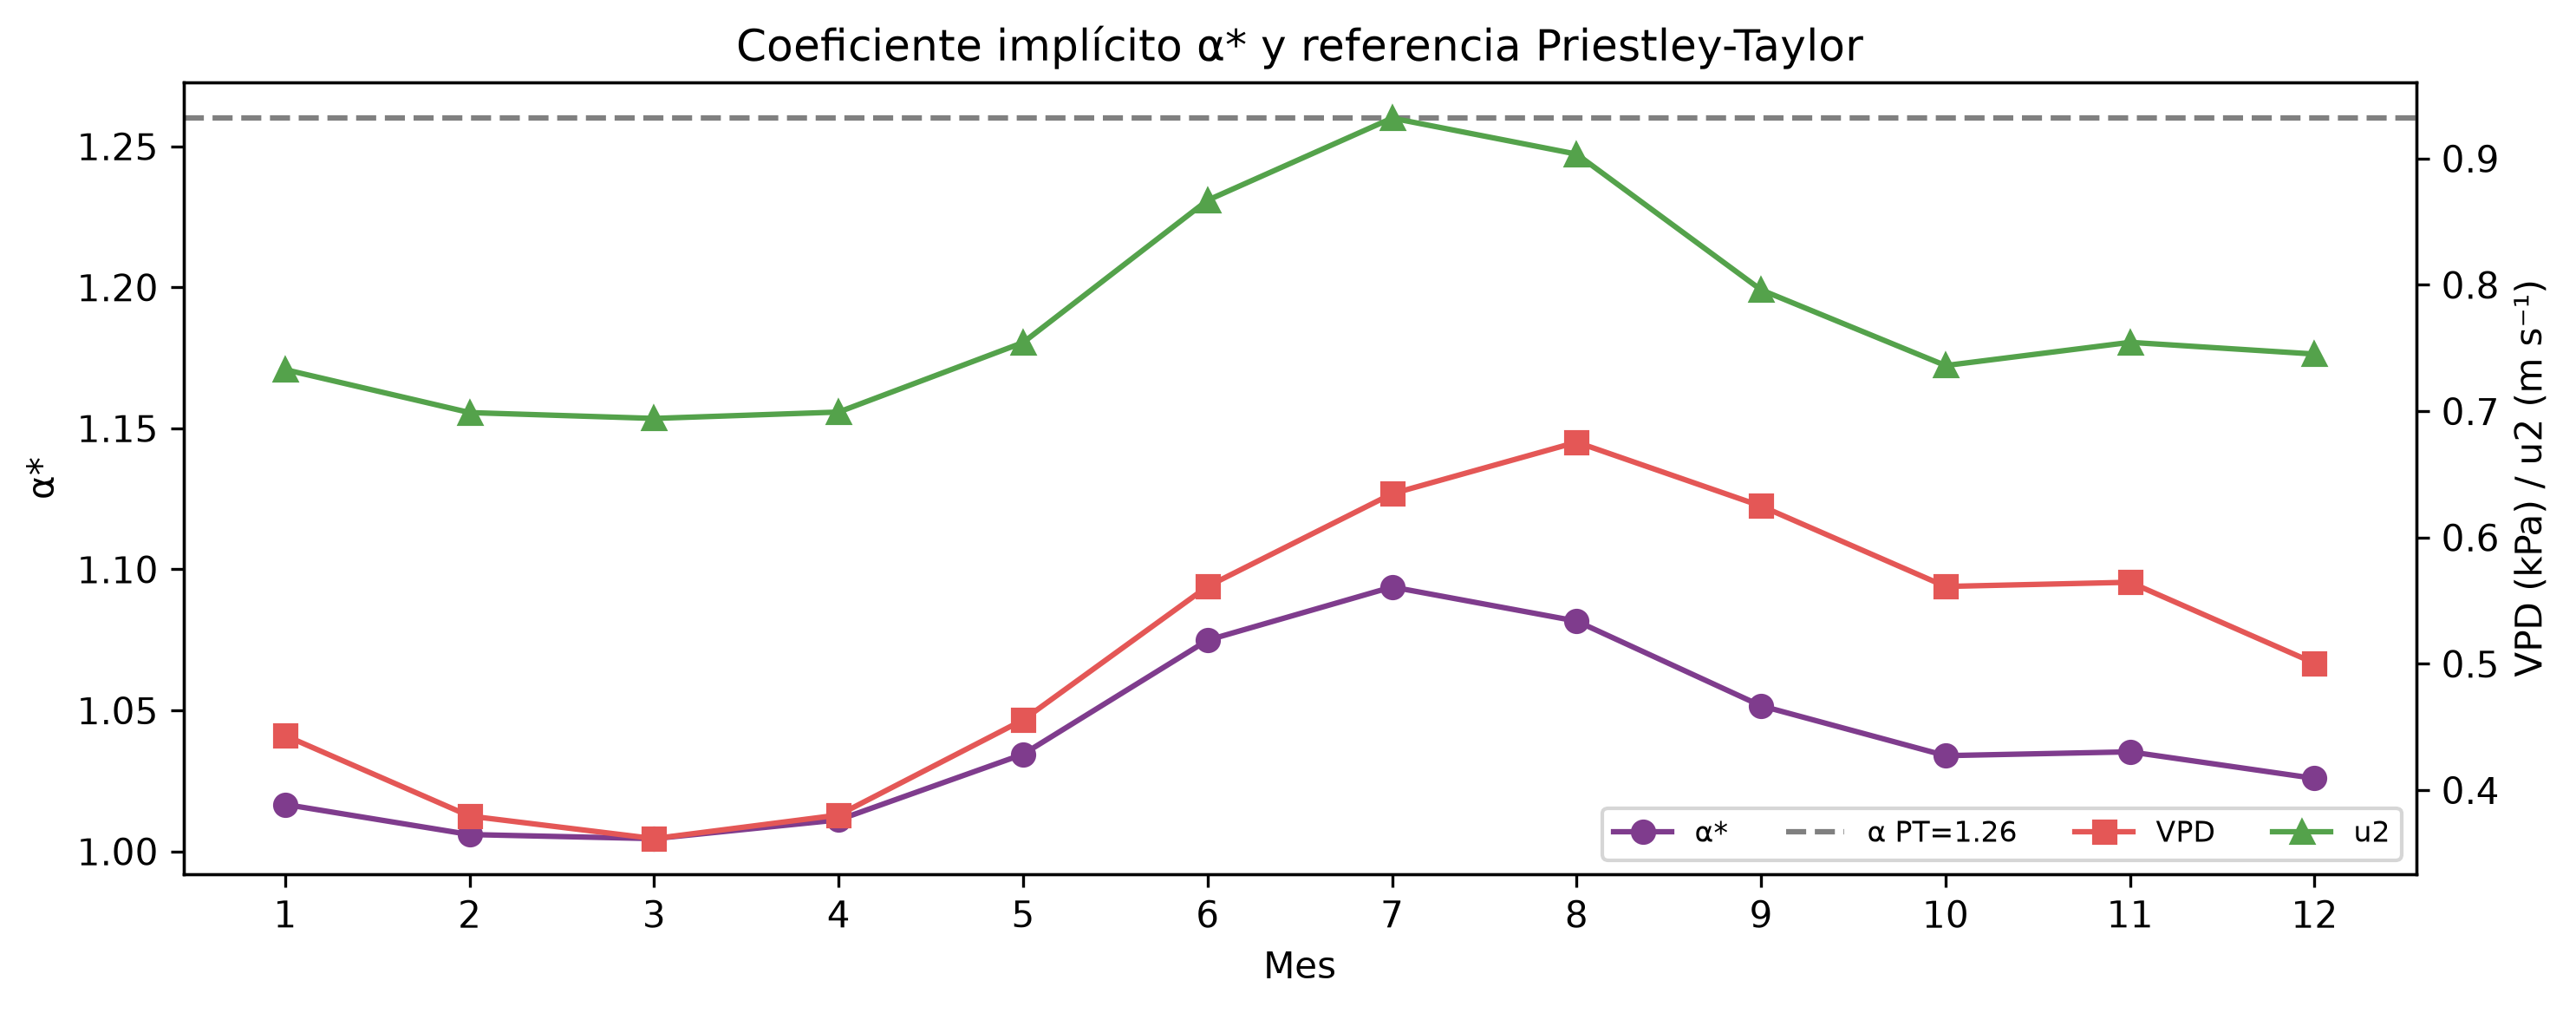
\includegraphics[width=0.85\linewidth]{1_1_demanda_atmosferica/figuras/1_1d_alpha_star_vpd_viento.png}
\nota{Promedios por mes calendario, 1981--2022, sobre el \CobEra\,\% de la cuenca.}
\end{figure}

\textbf{Qué mueve la demanda.} El coeficiente $\alpha^*$ varía entre \AlfaMin\ y \AlfaMax: es mínimo en la temporada húmeda y máximo en julio, cuando el déficit de vapor sube de \VPDMin\ a \VPDMax\ kPa y el viento se intensifica. Valores cercanos a 1 indican que, aun con la resistencia del pasto, el aire nunca está tan seco ni hay tanta advección como para que el término aerodinámico pese mucho. El experimento de sensibilidad lo confirma: $R_s-10$\,\% reduce la ETo en \SensRs\ mm/año (\SensPctRs\,\%), mientras que $u_2+10$\,\% la sube apenas \SensUdos\ mm/año y $e_a+10$\,\% la baja \SensEa\ mm/año. Un calentamiento de 1 °C con $e_a$ constante la sube \SensTunoEa\ mm/año (\SensPctTunoEa\,\%), pero con humedad relativa constante solo \SensTunoHR\ mm/año (\SensPctTunoHR\,\%): cerca de un tercio de la respuesta al calentamiento depende de lo que pase con la humedad. Thornthwaite responde a +1 °C con un \SensThornTuno\,\%, casi el doble que FAO-56 con humedad relativa constante, aunque no incluye la radiación, que es el forzante dominante; es la exageración de la respuesta térmica que advierten \textcite{milly2016}.

\textbf{Método simple recomendado.} El árbol de decisión de la sección 7 de las notas del curso \parencite{hoyos2026} indica, en su paso 4, que con solo temperaturas máxima y mínima se use Hargreaves--Samani, ``idealmente calibrado con una estación completa cercana''; Thornthwaite u Oudin quedan para el caso de solo temperatura media mensual (paso 6), conscientes de su sesgo. Los resultados de la cuenca respaldan esa elección: Hargreaves recoge el control radiativo a través del rango térmico, su error está dentro de la dispersión de las pruebas en 7 de los 12 meses y su respuesta al calentamiento es parecida a la de FAO-56, mientras que Thornthwaite la exagera. La calibración que recomienda el árbol funciona: con el coeficiente ajustado en 1981--2001 (\HSkCal\ en lugar de 0,0023), el MAE del periodo de validación 2002--2022 baja de \HSmaeValOrig\ a \HSmaeValCal\ mm/mes y el sesgo queda en \HSsesgoValCal\,\%. Calibrado con todo el periodo (\HSkTot), su MAE es de \HSmaeTot\ mm/mes, menor que el de Makkink. La calibración corrige el nivel, pero no la forma del ciclo: queda una sobrestimación de \HScalHum\ mm/mes en enero--marzo y una subestimación de \HScalSeco\ mm/mes en junio--septiembre, por la misma omisión del término aerodinámico.

\textbf{Verificación de unidades.} 146 W/m$^2$ de calor latente equivalen a $146\times3600/2{,}45\times10^6=0{,}215$ mm/h, es decir 5,15 mm/d; el valor de 3,52 mm/h de \textcite[sec.~10.3]{shaw2010} es unas 16 veces mayor y corresponde a mezclar horas con días. Un milímetro por día equivale a 28,4 W/m$^2$.

\subsection{Punto 1. La evapotranspiración real}

\textbf{Balance y su incertidumbre.} Con $P_L$, el balance da $ET=\ETbalL$ mm/año; con $P_I$, apenas \ETbalI\ mm/año. La diferencia viene de la precipitación: IMERG da \DifPLPI\ mm/año menos que PISCOp, lo que es coherente con la subestimación de la lluvia orográfica por los productos satelitales en los Andes. Con una incertidumbre de caudal de $\pm15$\,\%, la propagación da $\sigma_{ET}=\SigmaET$ mm/año (\SigmaETpct\,\% de la ET), de los cuales \SigmaP\ mm/año vienen de la precipitación y solo \SigmaQ\ del caudal: el sesgo de la lluvia pasa entero a la ET. Con $P_I$ el balance no es interpretable, porque la ET queda por debajo de una desviación estándar.

\textbf{Techo energético.} La radiación neta real equivale a \RnLambda\ mm/año; la fracción evaporativa del balance es \FEbal\ y ningún año supera el techo, de modo que no hay indicios de advección de energía a escala de cuenca.

\textbf{Productos.} GLEAM (\ETgleam\ mm/año) y MOD16 (\ETmod\ mm/año) superan al balance con $P_L$ en un \SobreGleam\ y un \SobreMod\,\%. Tres explicaciones compiten: (1) PISCOp subestima la lluvia de las partes altas, lo que reduciría el balance; (2) los trasvases desde el Chotano y el Conchano aumentan el caudal medido sin aumentar la lluvia de la cuenca, lo que también reduce $P-Q$; (3) los productos sobrestiman la ET en relieve complejo. Las dos primeras actúan en la misma dirección y son verificables con los volúmenes trasvasados. No hay torres de flujo representativas: la más cercana está a 206 km, en bosque amazónico de baja altitud.

\subsection{Punto 1. ¿Manda la energía o el agua?}

\begin{figure}[H]
\caption{Cociente mensual entre la evapotranspiración real de los productos y la ETo}
\label{fig:regimen}
\centering
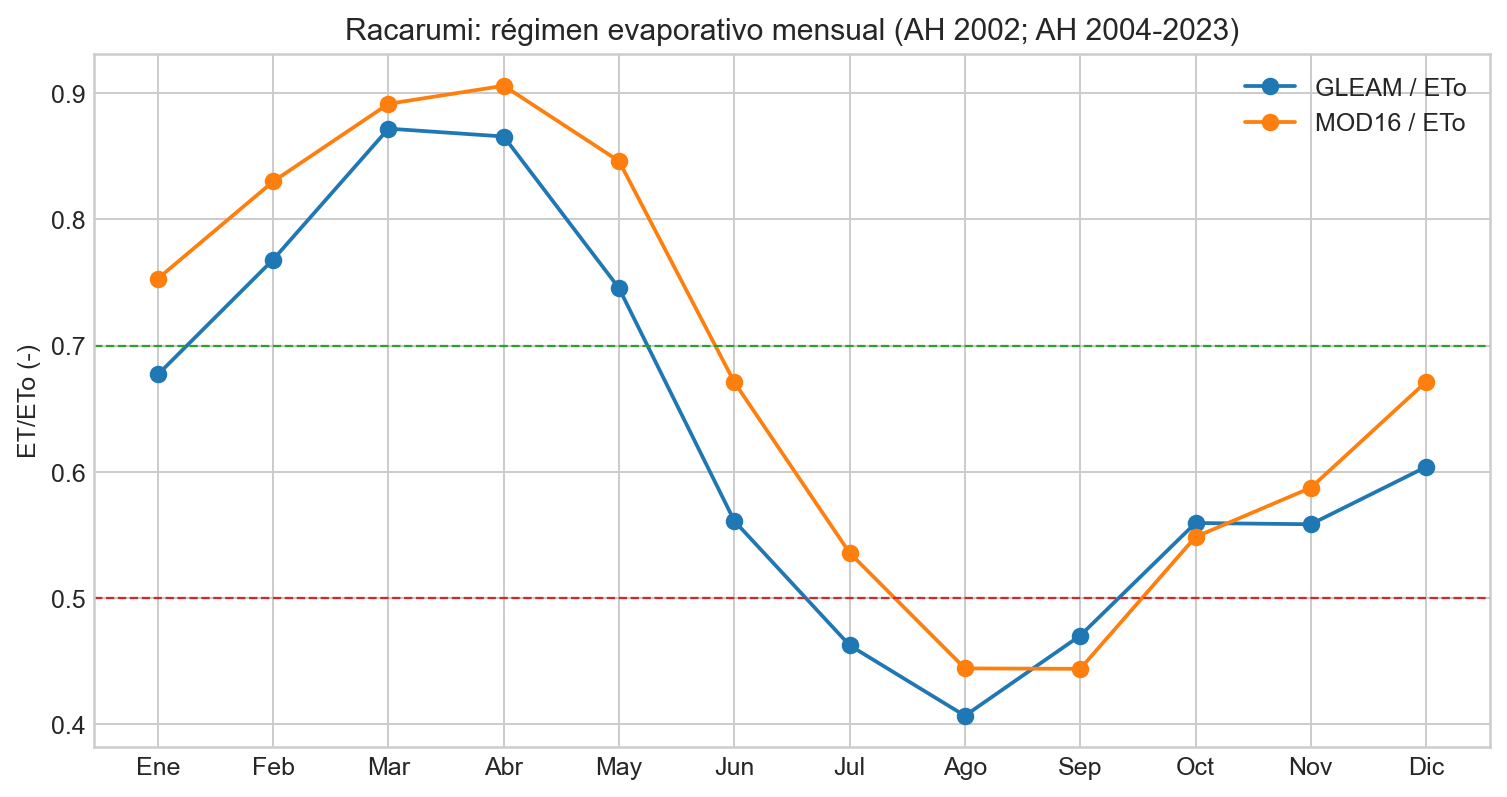
\includegraphics[width=0.8\linewidth]{1_3_regimen_evaporativo/figuras/1_3_integracion_1_3_1_ET_sobre_ETo_mensual.png}
\nota{GLEAM v4.3a y MOD16A2GF v6.1, años hidrológicos 2002 y 2004--2023.}
\end{figure}

\textbf{Régimen mensual.} Se clasificó un mes como limitado por energía si $ET/\mathrm{ETo}\geq0{,}7$ y $ET/P<1$, limitado por agua si $ET/\mathrm{ETo}<0{,}55$ o $ET/P>1$, y de transición en los demás casos. De enero a abril $ET/\mathrm{ETo}$ está entre \EToHumMin\ y \EToHumMax: meses limitados por energía, que coinciden con la temporada húmeda de la Tarea 1. De junio a septiembre baja a \EToSecMin--\EToSecMax\ y la ET supera a la lluvia del mes (figura~\ref{fig:regimen}): esa agua sale de la humedad del suelo almacenada en la temporada húmeda, que baja de 0,39 a 0,26 m$^3$/m$^3$, y posiblemente del riego con agua trasvasada. Mayo y octubre a diciembre son de transición.

\textbf{Humedad del suelo.} La fracción evaporativa crece con la humedad de la zona de raíces ($r=\CorrFEg$ con GLEAM y \CorrFEm\ con MOD16). Un ajuste por tramos sugiere un cambio de pendiente cerca de \KnotG--\KnotM\ m$^3$/m$^3$, que interpretamos como un umbral exploratorio: con una resolución de 9 km y sin mediciones de campo no es un umbral físico demostrado \parencite[sec.~6.8]{dingman2015}.

\textbf{Budyko.} Con $P_L$ y la ET de los productos, el índice de aridez $\phi=\mathrm{ETo}/P$ es \PhiAr, en plena transición entre los límites de energía y de agua, y el índice evaporativo es \EIg\ (GLEAM) y \EIm\ (MOD16), por encima de la curva de \textcite{budyko1974} (\BudyEI). Los parámetros de Fu son $\omega=\OmG$ y \OmM, cercanos al valor medio mundial. La cuenca evapora algo más que lo que su aridez predice. Lo atribuimos a dos rasgos propios: la humedad del suelo acumulada en la temporada húmeda sostiene la ET en los meses secos, y el riego con agua trasvasada añade agua que no está en $P$. La estacionalidad juega en contra (la lluvia llega cuando la radiación es moderada), lo que limita esa distancia. Con $P_I$ el índice de aridez sería \PhiI\ y $ET/P>1$, físicamente imposible: confirma que IMERG no sirve para el balance de esta cuenca.

\textbf{Elasticidad.} La elasticidad teórica de Fu es \ElasG--\ElasM: un cambio de 10\,\% en la lluvia cambiaría el caudal en un 20\,\%. La empírica es menor (1,5, con intervalo de 0,5 a 2,2), lo que concuerda con un sistema regulado por trasvases y bocatomas que amortiguan la respuesta del caudal.

\textbf{Relación complementaria.} En los años húmedos la ET es mayor (\ETHumG\ frente a \ETSecoG\ mm/año con GLEAM) y la ETo menor (\EToHumedo\ frente a \EToSeco\ mm/año); la correlación entre la lluvia anual y la ETo es \CorrPETo. Es lo que predice la relación complementaria \parencite{bouchet1963,brutsaert1998}: cuando la superficie se seca, el aire se calienta y se seca y la demanda sube. La explicación alternativa es la nubosidad: los años húmedos son más nublados y reciben menos radiación. Con los datos disponibles no se pueden separar.

\textbf{Síntesis del régimen.} La cuenca tiene un régimen evaporativo estacional mixto: limitado por energía en la temporada húmeda, por agua en la seca y en la transición en el promedio multianual. Esto confirma y precisa la hipótesis de la Tarea 1 de que el agua vuelve a la atmósfera sobre todo durante y justo después de la temporada húmeda.

\subsection{Punto 1. Cambios en la demanda}

La ETo FAO-56 aumentó \TendETo\ mm/año por año entre 1981 y 2022 ($p=\pETo$), y Thornthwaite \TendTh\ ($p=\pTh$); el signo y la significancia se mantienen en los 49 escenarios de robustez. La atribución (figura~\ref{fig:atrib}) asigna \AtrT\ mm/año por año a la temperatura, que subió \TendT\ °C por década, \AtrRs\ a la radiación solar, \AtrEa\ a la humedad y \AtrUdos\ al viento. La suma (\AtrSuma) reproduce la tendencia directa con un residuo de \AtrRes\ mm/año por año, que mide las interacciones y la no linealidad.

\begin{figure}[H]
\caption{Contribución de cada forzante a la tendencia de la ETo FAO-56}
\label{fig:atrib}
\centering
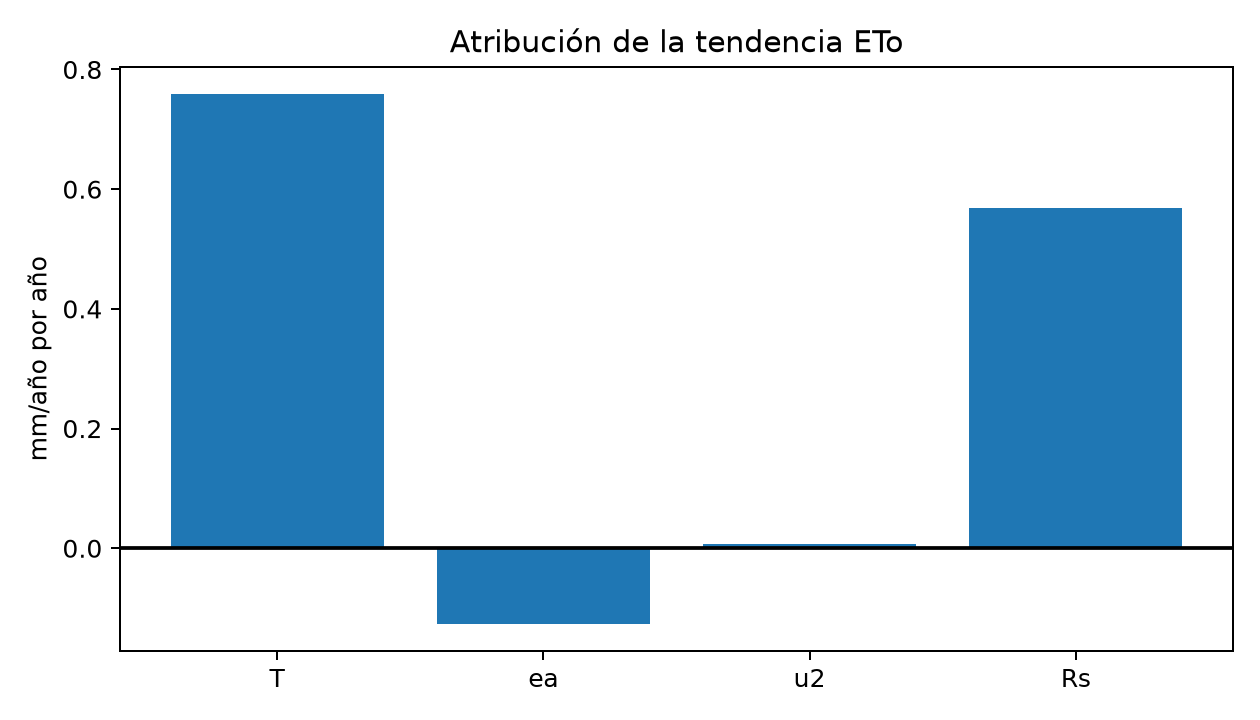
\includegraphics[width=0.7\linewidth]{1_4_cambios_demanda_evaporativa/figuras/1_4_2_contribuciones.png}
\nota{Sensibilidad numérica de la ecuación diaria multiplicada por la tendencia de Sen de cada forzante, 1981--2022.}
\end{figure}

\textbf{Paradoja del tanque.} No hay datos de tanque evaporímetro en la cuenca. Aquí no aparece la paradoja: Thornthwaite crece la mitad que FAO-56, no más, porque la radiación también aumentó y la humedad solo compensa una parte. La tendencia de la radiación debe tomarse con cautela: puede reflejar cambios reales de nubosidad o cambios en los datos asimilados por el reanálisis. Una tendencia estadística no identifica una causa \parencite{roderick2002,mcvicar2012}.

\subsection{Punto 1. El paisaje: gradiente altitudinal}

\begin{figure}[H]
\caption{ETo y evapotranspiración real por banda de elevación}
\label{fig:gradiente}
\centering
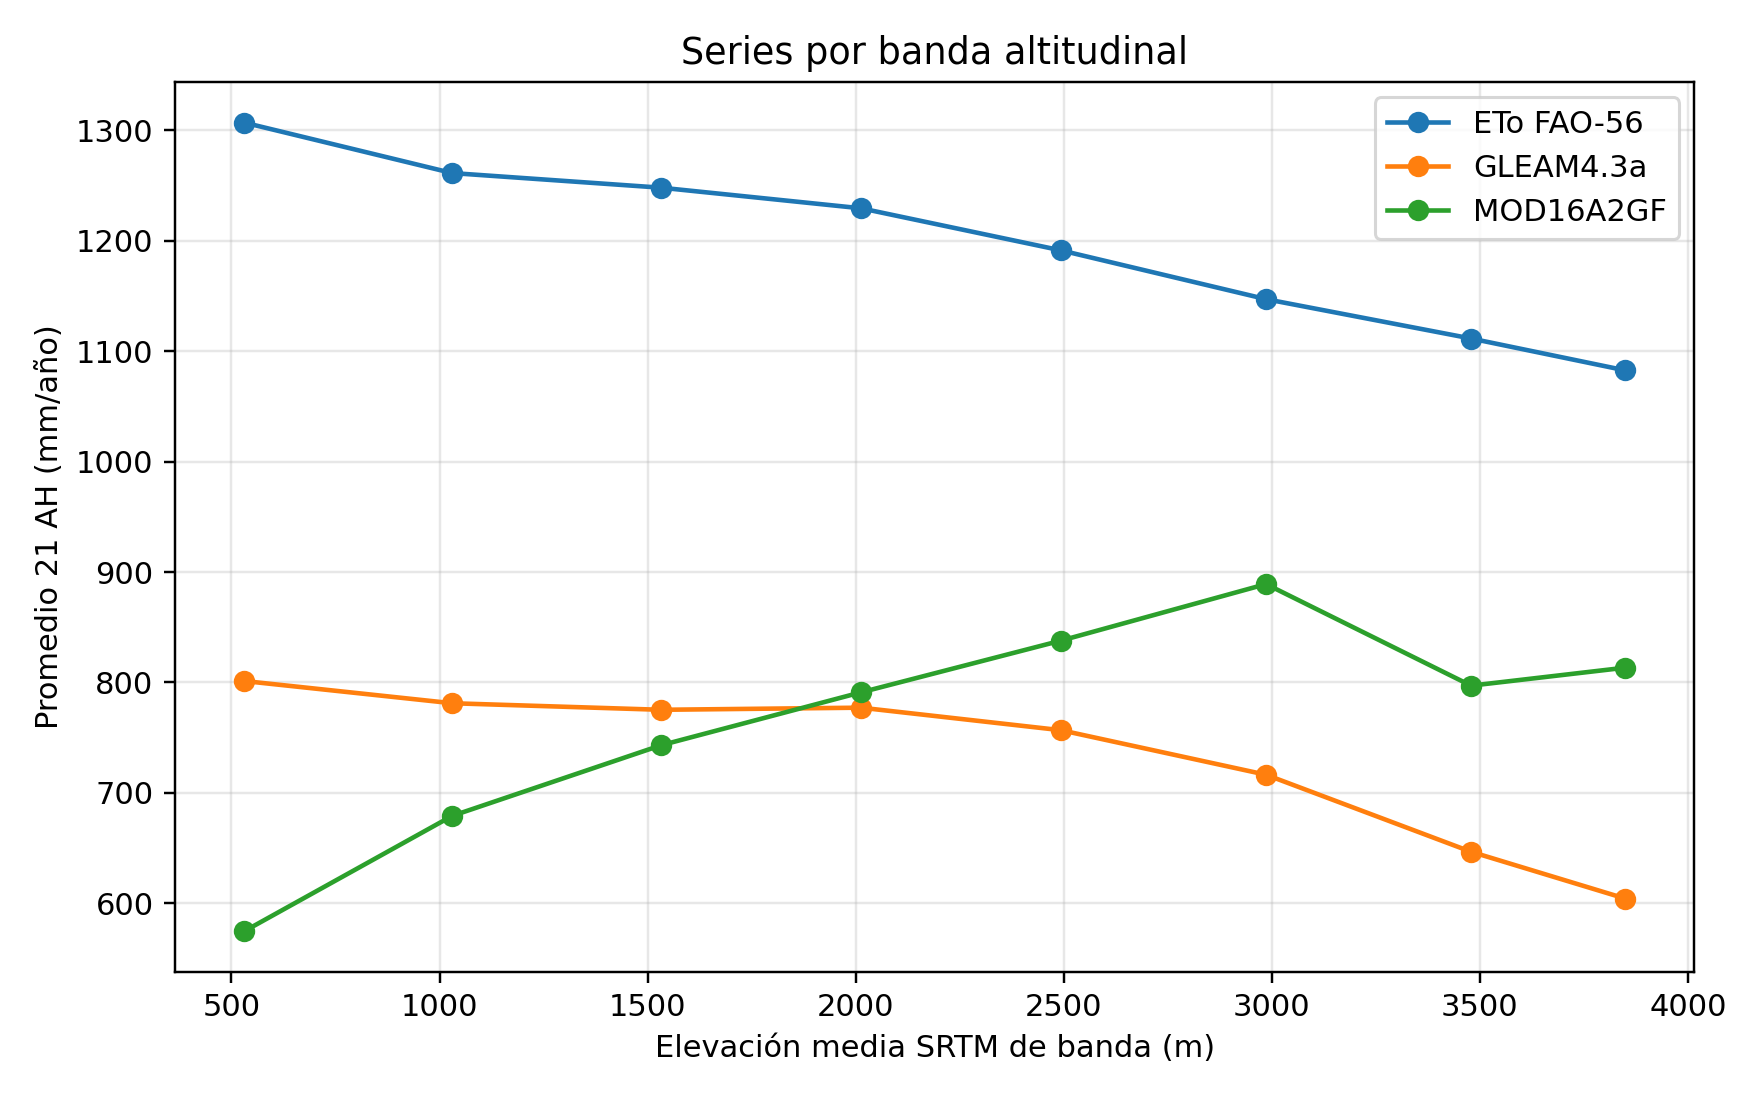
\includegraphics[width=0.75\linewidth]{1_5_paisaje/1_5_gradiente_multianual_productos.png}
\nota{Bandas de 500 m con el DEM SRTM; promedios de los años hidrológicos 2002 y 2004--2023.}
\end{figure}

La ETo disminuye de forma monótona con la altura, de \EToBajo\ mm/año en la banda más baja a \EToAlto\ en la más alta, porque el enfriamiento con la altura pesa más que el aumento de la radiación. Los dos productos de ET real discrepan en el signo del gradiente (figura~\ref{fig:gradiente}): GLEAM baja de \GlBajo\ a \GlAlto\ mm/año, siguiendo a la demanda, mientras que MOD16 sube de \ModBajo\ hasta un máximo de \ModMax\ mm/año en la banda de \ModMaxBanda\ y luego baja. El máximo intermedio de MOD16 es compatible con lo descrito por \textcite{dejong2005}: en las laderas bajas y secas la ET está limitada por agua y en las partes altas por energía, y la franja intermedia de bosque montano y jalca combina humedad y energía suficientes. GLEAM no lo muestra porque su estrés hídrico se calcula a 0,1° y no resuelve la ladera. Un producto de 9 km mezcla en una celda bandas separadas por más de 1000 m, así que el gradiente real es incierto.

\subsection{Síntesis del punto 1}

\begin{figure}[H]
\caption{Esquema conceptual actualizado del balance de la cuenca Racarumi}
\label{fig:esquema}
\centering
\begin{tikzpicture}[node distance=1.2cm, every node/.style={font=\small}, box/.style={draw, rounded corners, align=center, minimum width=3.4cm, minimum height=1cm}]
\node[box, fill=blue!8] (p) {Precipitación\\ $P_L$ = \PL\ mm/año\\ (IMERG: \ETbalI\ + \Qmed)};
\node[box, fill=orange!10, right=3.6cm of p] (eto) {Demanda ETo\\ \EToAnual\ mm/año\\ techo $R_n/\lambda$ = \RnLambda};
\node[box, fill=green!10, below=1.4cm of p] (s) {Suelo (zona de raíces)\\ 0,39 $\to$ 0,26 m$^3$/m$^3$\\ húmeda $\to$ seca};
\node[box, fill=green!10, right=3.6cm of s] (et) {ET real\\ balance \ETbalL\ $\pm$ \SigmaET\\ productos \ETgleam--\ETmod};
\node[box, fill=blue!8, below=1.4cm of s] (q) {Caudal en Racarumi\\ \Qmed\ mm/año};
\node[box, fill=gray!10, right=3.6cm of q] (t) {Trasvases\\ Chotano--Conchano\\ (entrada no medida)};
\draw[-{Latex}] (p) -- (s);
\draw[-{Latex}] (s) -- node[below, font=\footnotesize]{jun--sep: $ET>P$} (et);
\draw[-{Latex}, dashed] (eto) -- node[right, font=\footnotesize]{limita ene--abr} (et);
\draw[-{Latex}] (s) -- (q);
\draw[-{Latex}] (t) -- (q);
\draw[-{Latex}, dashed] (t) -- node[right, font=\footnotesize]{riego} (et);
\end{tikzpicture}
\nota{Flujos en mm/año, promedios multianuales. Los trasvases no están cuantificados.}
\end{figure}

La atmósfera demanda unos \EToAnual\ mm/año, controlados sobre todo por la radiación. La cuenca devuelve entre \ETbalL\ mm/año (balance, $\pm$\SigmaET) y \ETmod\ mm/año (productos), con una incertidumbre que viene casi toda de la lluvia. La energía manda de enero a abril y el agua de junio a septiembre. La demanda creció por el calentamiento y el aumento de la radiación. Lo que distingue a la cuenca es su gradiente altitudinal, con un posible máximo de ET a media ladera. Lo observado es el caudal; la lluvia, la ETo y la ET de los productos son estimaciones; la influencia de los trasvases y el umbral de humedad son hipótesis de interpretación (figura~\ref{fig:esquema}).

% ------------------------------------------------------------------ punto 2
\subsection{Punto 2. Datos y extremos}

\textbf{Calidad de la serie.} Los \NAnios\ años hidrológicos (2006--2025) tienen una completitud mínima de \CompletMin\,\% y no hay incoherencias entre duraciones. El máximo de 24 h móviles supera a la mayor lluvia diaria de reloj del mismo año en una proporción coherente con la corrección de Weiss. El mayor evento del registro, el 24 de julio de 2013 (81 mm en 1 h, 111 mm en el día), muestra la forma de una tormenta convectiva: sube y baja en 10 minutos consecutivos, con código de calidad 3, sin vacíos previos ni valores repetidos. Para descartar un error del sensor, el evento se contrastó con datos independientes (figura~\ref{fig:evento2013}). El radar muestra una celda convectiva centrada en la estación: \EvRadarEst\ mm en la hora más intensa y \EvRadarTresEst\ mm en tres horas en la celda de 1 km de la estación, que es la misma de la microcuenca, con un máximo de \EvRadarMaxVent\ mm a 5 km. Solo \EvAreaCuarenta\ km$^2$ superaron 40 mm. Los pluviómetros diarios reproducen el mismo patrón: el más cercano al núcleo según el radar, Bühlerzell (a \EvBuhlerKm\ km, \EvRadarBuhler\ mm/h en el radar), midió \EvBuhler\ mm; Abtsgmünd-Neubronn \EvNeubronn\ y Göggingen \EvGoggingen\ mm, y Heubach y Aalen, más lejos, \EvHeubach\ y \EvAalen\ mm. Las estaciones de 10 minutos registraron la misma tormenta a la misma hora, pero en su periferia: \EvGmundHora\ mm/h en Schwäbisch Gmünd y \EvEllwHora\ mm/h en Ellwangen. El evento es real y local: la estación quedó en el núcleo de una celda de pocos kilómetros, y por eso el pluviómetro registra más del doble que el radar, que promedia 1 km$^2$ y una hora. Se conservó como dato válido.

\begin{figure}[H]
\caption{Contraste del evento del 24 de julio de 2013}
\label{fig:evento2013}
\centering
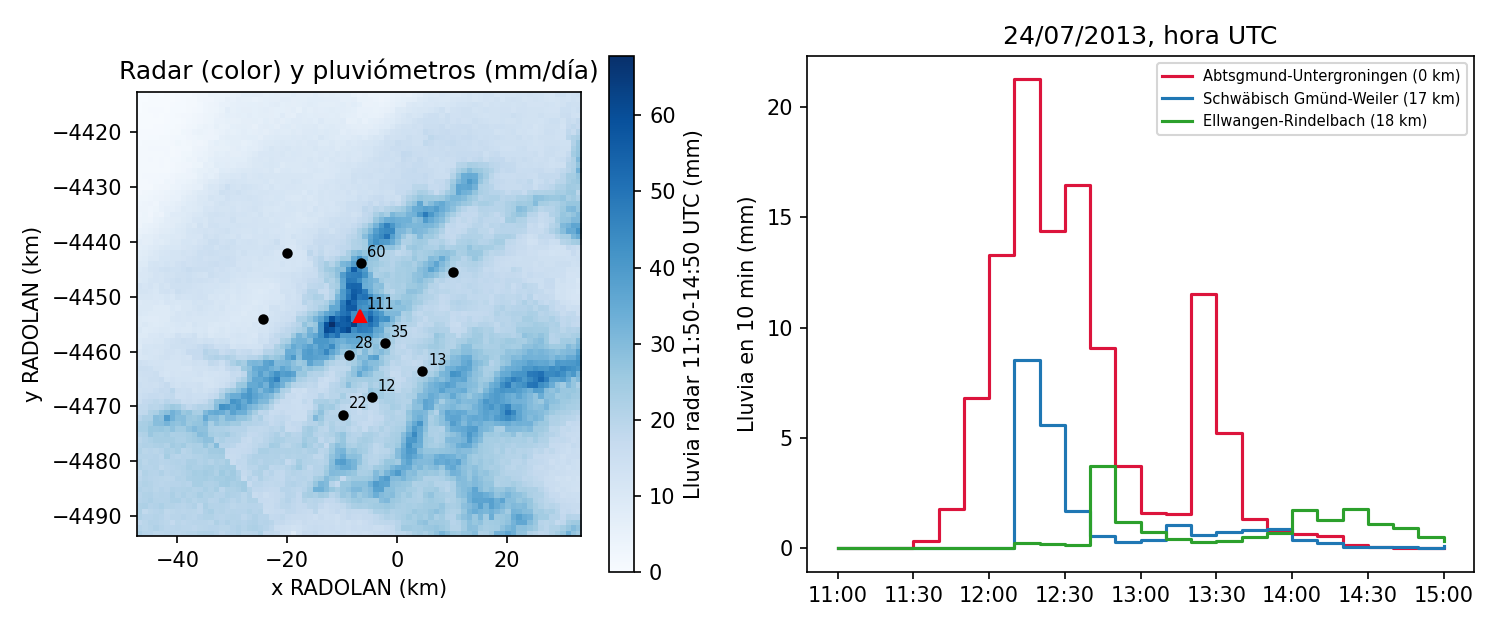
\includegraphics[width=\linewidth]{evento_2013_contraste.png}
\nota{Izquierda: lluvia RADOLAN RW entre 11:50 y 14:50 UTC (color); triángulo rojo: estación 00020; puntos: pluviómetros con su lluvia diaria en mm. Derecha: lluvia de 10 minutos en la estación y en las dos vecinas con registro largo.}
\end{figure}

\begin{figure}[H]
\caption{Microcuenca, estación pluviométrica y salida}
\label{fig:mapa}
\centering
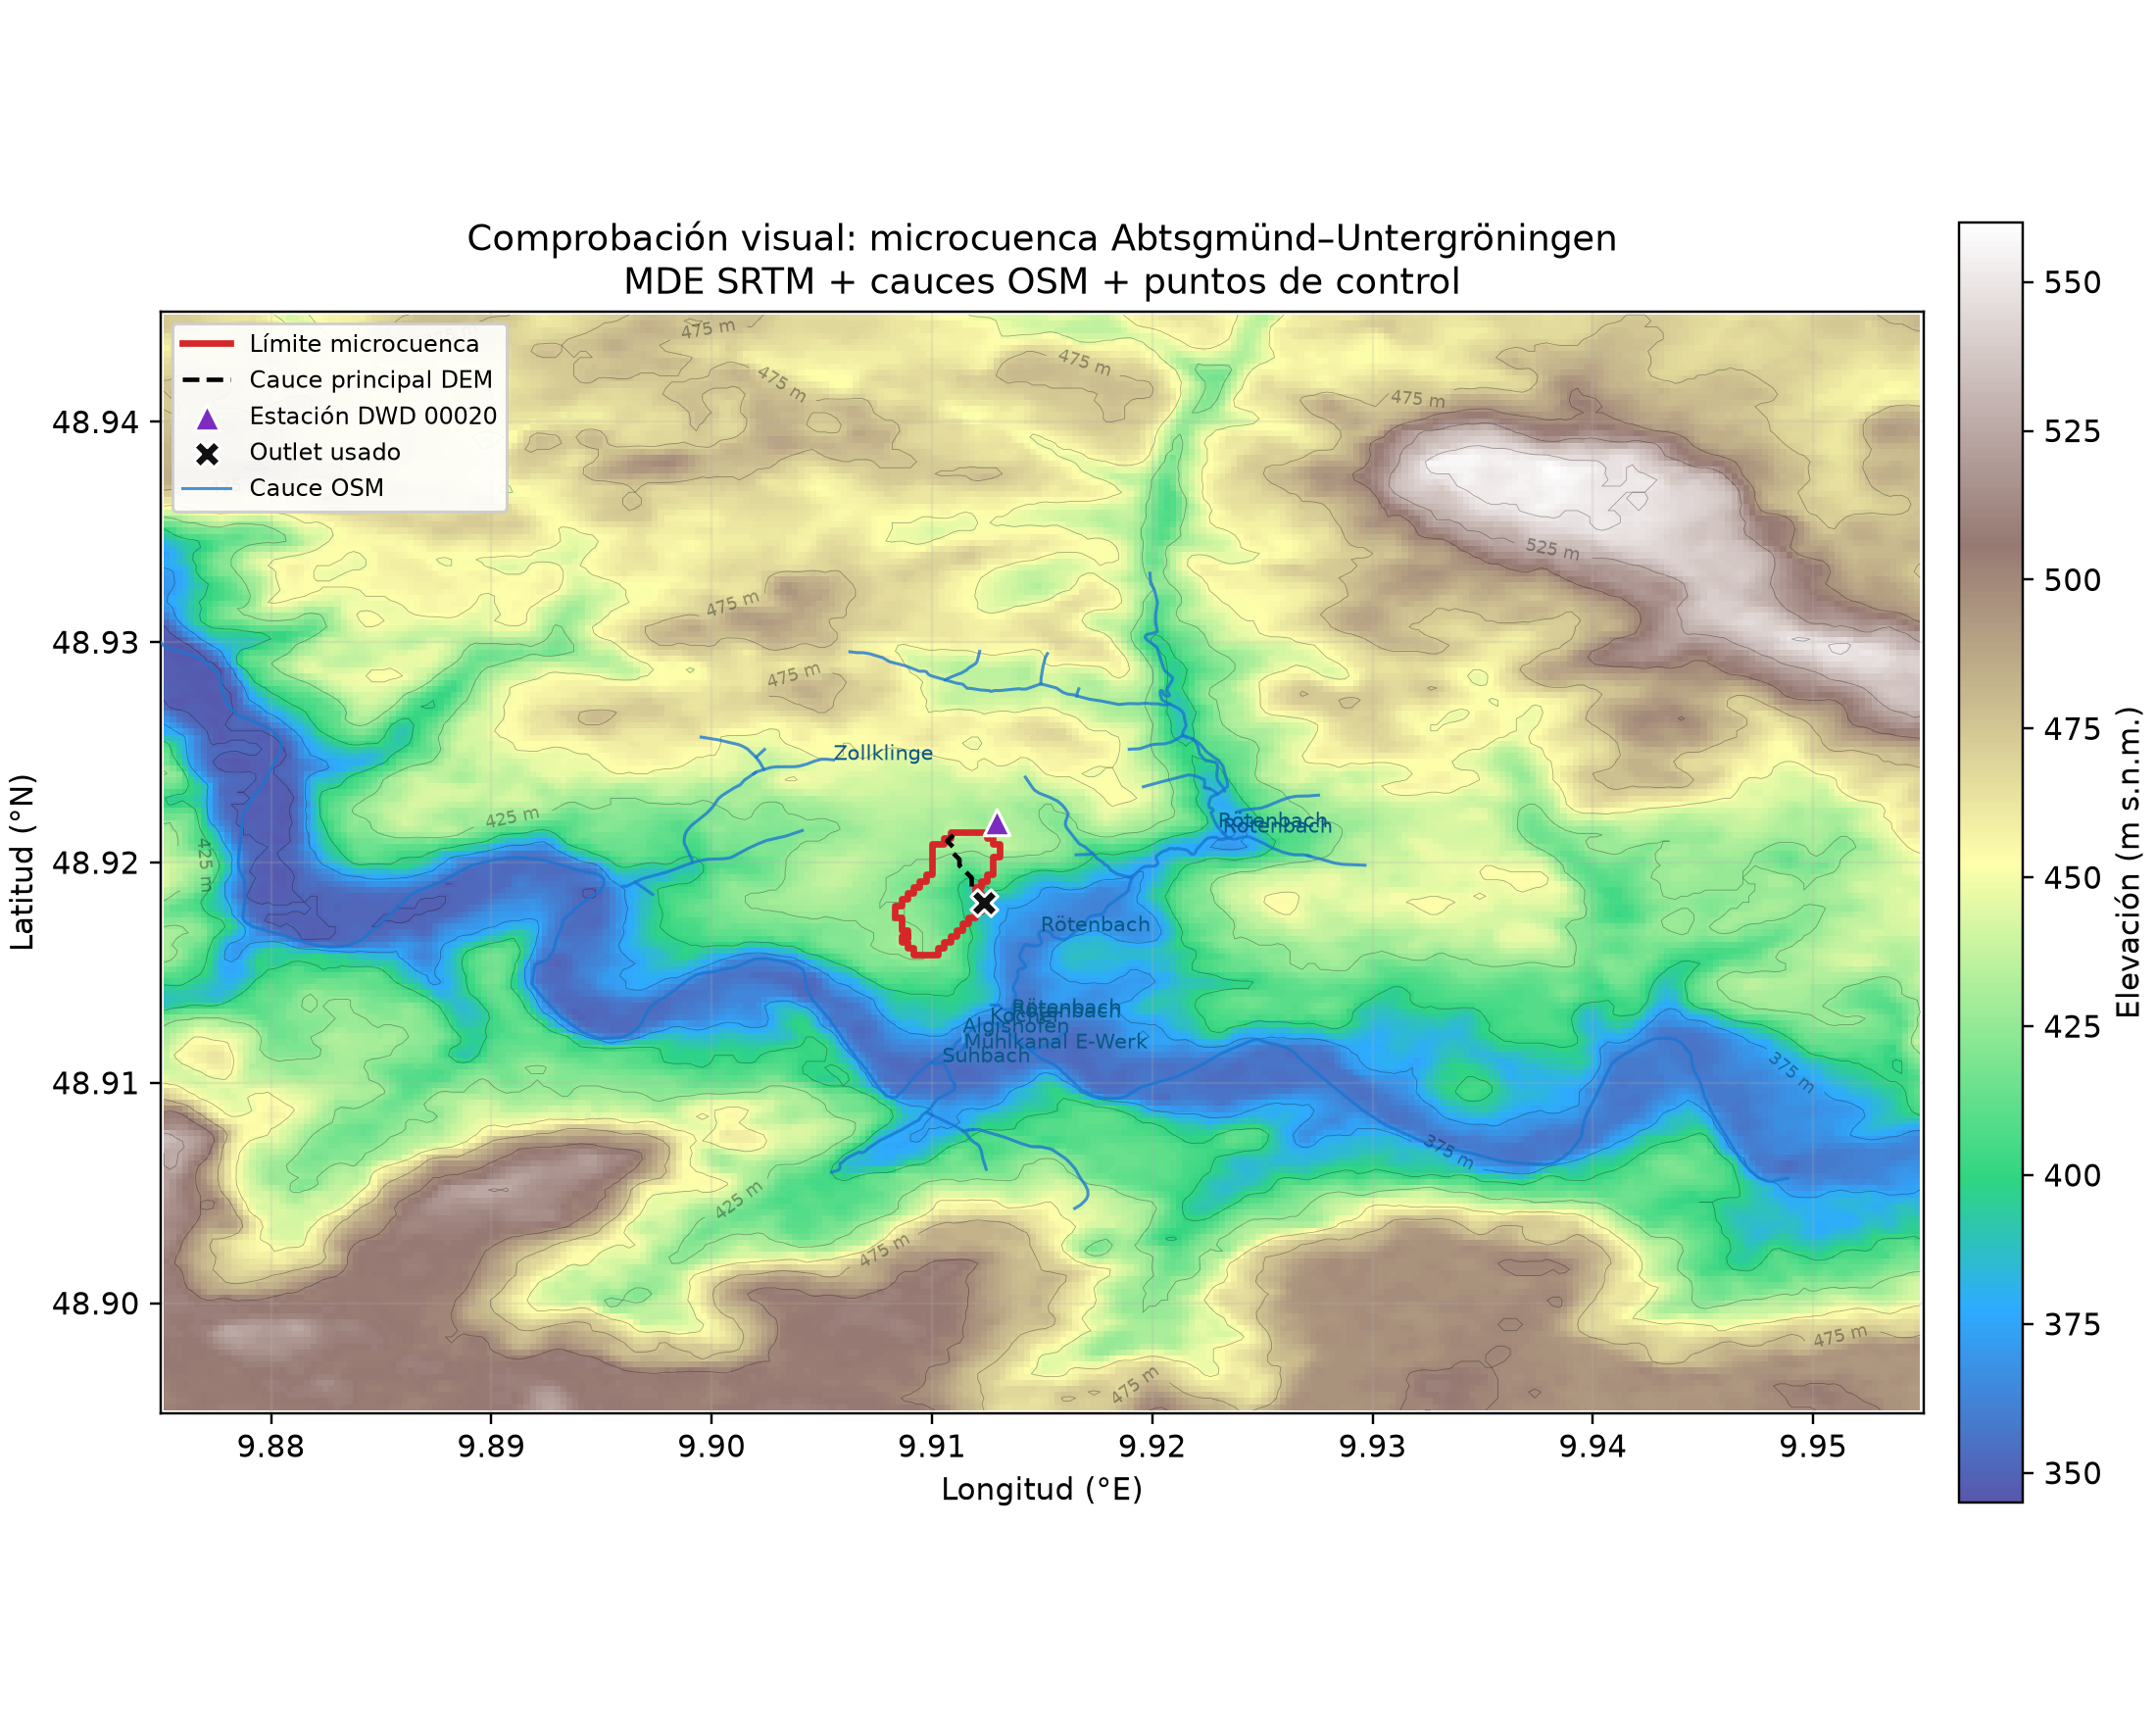
\includegraphics[width=0.8\linewidth]{mapa_revision_visual.png}
\nota{DEM SRTM de 1''. La salida se ubicó en el extremo aguas abajo del cauce derivado del DEM; no coincide con una obra existente.}
\end{figure}

\textbf{Distribuciones.} Las pruebas no rechazan ninguna distribución (tabla~\ref{tab:cuantiles}). Con 20 datos no distinguen bien familias parecidas: no rechazar no es demostrar. El diagrama de L-momentos (figura~\ref{fig:lmom}) es más informativo: las duraciones de 30 min a 24 h tienen L-asimetrías de 0,38 a 0,51, por encima de Gumbel (0,17), lo que indica una cola más pesada que Gumbel. Esa forma la determina sobre todo el evento de 2013: sin él, el cuantil de 100 años de 1 h baja de \QhoraTcien\ a \SinHoraTcien\ mm. Por eso la elección no se basó en el menor estadístico, sino en la estabilidad de los cuantiles altos, con GEV-GMLE como compromiso entre una cola pesada y una forma estable.

\begin{table}[H]
\caption{Cuantiles de profundidad (mm) y bondad de ajuste para 10 minutos y 1 hora}
\label{tab:cuantiles}
\centering\footnotesize
\begin{tabular}{llrrrrrrrrr}
\toprule
$d$ & Modelo & $T=2$ & 5 & 10 & 25 & 50 & 100 & $p$ KS & $p$ CvM & PPCC \\
\midrule
\csname @@input\endcsname ../../productos/punto2/final/tablas_tex/cuantiles.tex 
\bottomrule
\end{tabular}
\nota{Máximos anuales con corrección de Weiss. GMLE: máxima verosimilitud generalizada; MV: máxima verosimilitud; LM: L-momentos. Las siete duraciones están en \texttt{productos/punto2/final/tablas/cuantiles\_todas\_duraciones.csv}.}
\end{table}

\begin{figure}[H]
\caption{Diagrama de razones de L-momentos de los máximos anuales}
\label{fig:lmom}
\centering
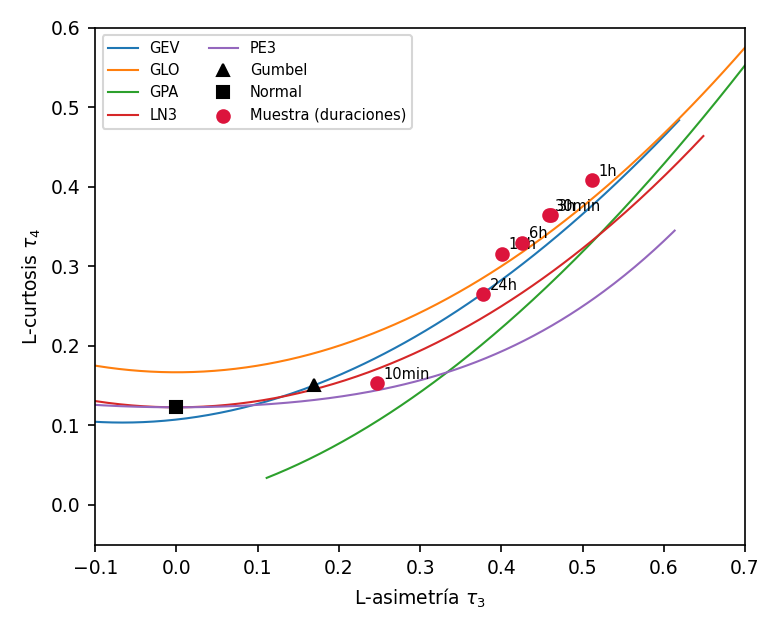
\includegraphics[width=0.62\linewidth]{lmomentos_diagrama.png}
\end{figure}

\textbf{Incertidumbre y tendencia.} El intervalo bootstrap de 95\,\% se ensancha rápido cuando $T$ supera a $N$: para 10 minutos y $T=100$ años su ancho es el \AnchoTcien\,\% del cuantil (figura~\ref{fig:ancho}). Más allá de $T\approx2N=40$ años el cuantil depende casi por completo de la forma supuesta de la cola. Mann--Kendall no encuentra tendencia significativa en ninguna duración ($p>0{,}25$); eso no garantiza que el clima futuro sea estacionario.

\begin{figure}[H]
\caption{Ancho relativo del intervalo de confianza de 95\,\% frente a $T/N$}
\label{fig:ancho}
\centering
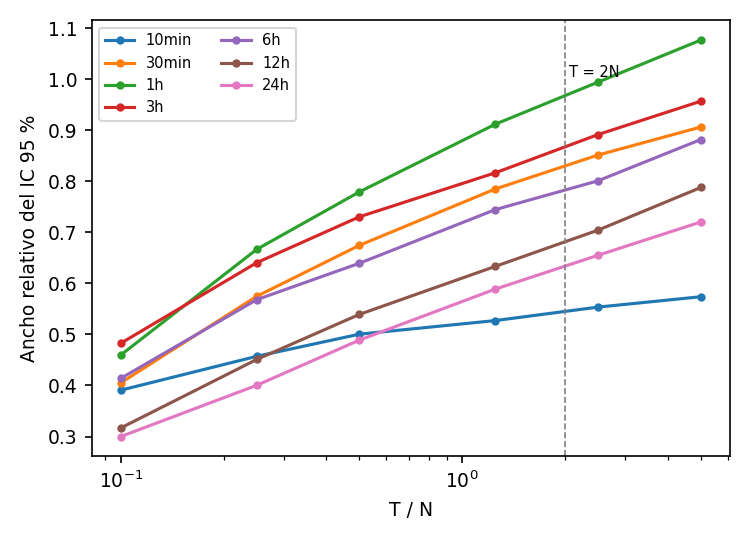
\includegraphics[width=0.6\linewidth]{ancho_relativo_ic.png}
\end{figure}

\subsection{Punto 2. Curvas IDF}

La forma de Koutsoyiannis ajusta los cuantiles GEV-GMLE con $\theta=\IDFtheta$ h, $\eta=\IDFeta$, RMSE de \IDFrmse\ mm/h, error relativo máximo de \IDFerr\,\% y $R^2$ logarítmico de \IDFrdos. Las curvas no se cruzan y la profundidad crece con la duración. Son válidas entre 10 minutos y 24 horas y entre 2 y 100 años; por encima de 40 años la incertidumbre domina (figura~\ref{fig:idf}).

\begin{figure}[H]
\caption{Curvas IDF con bandas de confianza de 95\,\% y comparación con KOSTRA-DWD-2020}
\label{fig:idf}
\centering
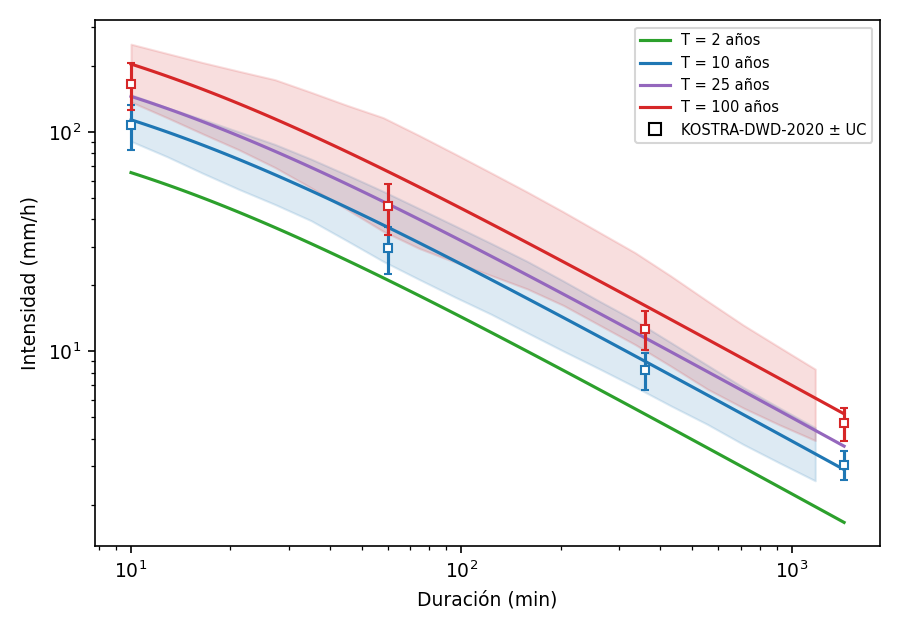
\includegraphics[width=0.75\linewidth]{idf_bandas_kostra.png}
\nota{Bandas bootstrap para $T=10$ y $T=100$ años. Cuadrados: KOSTRA-DWD-2020 en la celda de la estación con su incertidumbre (UC).}
\end{figure}

\begin{table}[H]
\caption{Comparación de la IDF local con KOSTRA-DWD-2020 (profundidades en mm)}
\label{tab:kostra}
\centering\small
\begin{tabular}{lrrrrr}
\toprule
Duración & $T$ & KOSTRA $\pm$ UC & Local & Local/KOSTRA & Local sin 2013 \\
\midrule
\csname @@input\endcsname ../../productos/punto2/final/tablas_tex/kostra.tex 
\bottomrule
\end{tabular}
\end{table}

\textbf{Comparación con KOSTRA.} Para periodos cortos la IDF local está dentro de la incertidumbre de KOSTRA; para 1 h y $T=100$ años es \RazonHoraTcien\ veces KOSTRA (\QhoraTcien\ frente a \KosHoraTcien\ mm, $\pm$\KosUCHoraTcien\,\%). La diferencia tiene dos causas. KOSTRA regionaliza estaciones vecinas y diluye el efecto de un evento aislado, mientras que la serie local de 20 años lo contiene. Además, KOSTRA representa una celda de 5 km, es decir una lluvia en parte areal. Sin el evento de 2013 el cuantil local (\SinHoraTcien\ mm) queda dentro de la incertidumbre de KOSTRA, por lo que la mayor parte de la diferencia es muestral y no un sesgo del pluviómetro. Las dos vecinas con registro largo lo confirman de forma independiente: con el mismo método (GEV-GMLE con Weiss), su cuantil de 1 h y 100 años es \VecGmundQcien\ mm en Schwäbisch Gmünd y \VecEllwQcien\ mm en Ellwangen, entre el valor local (\VecPropQcien\ mm) y KOSTRA. La cola pesada es en parte regional y en parte el efecto del evento de 2013 en la serie local. La correlación de Spearman entre los máximos anuales de 1 h de la estación y los de las vecinas es baja (\VecRhoGmund\ y \VecRhoEllw): a 17 km las tormentas convectivas de cada año son distintas, de modo que las vecinas sirven para verificar eventos y cuantiles, no para rellenar la serie. Para separar la reducción areal del sesgo del producto habría que comparar con varios pluviómetros dentro de la misma celda. Para 10 minutos, la duración más cercana a la de diseño, la IDF local está dentro de la incertidumbre de KOSTRA en todos los periodos de retorno (para $T=20$ años, la razón es \RazonDiezTveinte).

\textbf{Eventos recientes.} El máximo horario de 2021 (48,3 mm sin corregir) tiene un periodo de retorno de \TeventoVeintiuno\ años, con intervalo de \TeventoVeintiunoLo\ a más de 1000 años: un solo evento no permite hablar de cambio. El de 2013 tiene un periodo de retorno estimado de \TeventoTrece\ años, mayor que la longitud del registro.

\subsection{Punto 2. Problema A: alcantarilla}

\textbf{Microcuenca.} La microcuenca tiene \AreaMicro\ km$^2$, un cauce principal de \LongCauce\ m con pendiente de \PendCauce\ m/m y está a 414 m de la estación y 15 m más baja, en el mismo valle y con la misma exposición a las tormentas convectivas que llegan del oeste, por lo que la IDF del pluviómetro es aplicable (figura~\ref{fig:mapa}). La cobertura es 57\,\% bosque, 32\,\% pastizal y 11\,\% cultivo; con coeficientes de 0,30, 0,35 y 0,45 \parencite[tabla 15.1.1]{chow1988}, $C=\Cpre$. El área es tan pequeña que el factor de reducción areal es 1 \parencite{svensson2010}.

\textbf{Tiempo de concentración.} Kirpich da \tcKirpich\ min, el retardo del SCS \tcSCS\ min y Kerby \tcKerby\ min. Difieren cinco veces porque representan procesos distintos: Kirpich se calibró con cauces definidos y responde solo a la longitud y la pendiente; Kerby describe flujo superficial laminar sobre vegetación densa, y el SCS incorpora la cobertura y el suelo mediante el número de curva (CN = 75). Se adoptó el SCS: la microcuenca es en su mayoría bosque y pasto, sin un cauce permanente, y su valor queda dentro del rango de duraciones de la IDF. Kirpich exigiría extrapolar la IDF por debajo de la resolución de 10 minutos. \textit{La versión anterior del análisis daba 9,4 min para el SCS porque tenía intercambiadas la pendiente y la retención potencial en la fórmula.}

\textbf{Periodo de retorno.} La obra es una alcantarilla bajo una vía rural de tránsito intermedio; su falla es el rebose temporal de la vía, sin riesgo para vidas. La práctica recomienda 10 a 25 años para ese caso \parencite[tabla 13.1.1]{chow1988}. Con una vida útil de \Vida\ años y un riesgo aceptable de \RiesgoAcept\,\% de que el caudal de diseño se supere al menos una vez, el periodo de retorno requerido es \Treq\ años; se adoptó $T=\Tdis$ años, con un riesgo nominal de \RiesgoNom\,\%. \PENDIENTE{confirmar tipo de vía, vida útil y riesgo aceptable}

\textbf{Caudal y diámetro.} Con $i(t_c,T)=\Idis$ mm/h, el caudal de diseño es $Q_p=\Qp$ m$^3$/s. Con $n=0{,}013$ y $S_0=0{,}010$, el diámetro calculado es \Dcalc\ m y el comercial superior \Dcom\ m, con un factor de seguridad de \FS.

\begin{table}[H]
\caption{Sensibilidad del caudal y del diámetro}
\label{tab:sens}
\centering\footnotesize
\begin{tabular}{llrrr}
\toprule
Fuente & Escenario & $Q_p$ (m$^3$/s) & $D$ calculado (m) & $D$ comercial (m) \\
\midrule
\csname @@input\endcsname ../../productos/punto2/final/tablas_tex/sensibilidad.tex 
\bottomrule
\end{tabular}
\end{table}

\begin{figure}[H]
\caption{Rango del diámetro calculado por fuente de incertidumbre}
\label{fig:tornado}
\centering
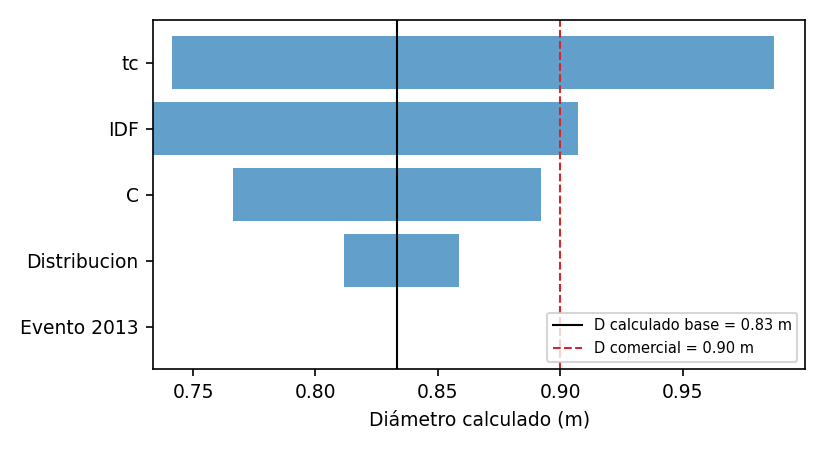
\includegraphics[width=0.7\linewidth]{tornado_2_4A.png}
\end{figure}

\textbf{Sensibilidad.} La tabla~\ref{tab:sens} y la figura~\ref{fig:tornado} ordenan las fuentes de incertidumbre por su efecto en el diámetro. La mayor es el tiempo de concentración: entre Kirpich y Kerby la intensidad de diseño cambia casi al doble. Le siguen el intervalo de confianza de la IDF y el coeficiente de escorrentía; la elección de la distribución y el evento de 2013 pesan menos a esta duración corta, porque la cola pesada afecta sobre todo a las duraciones de 30 min a 6 h. Esto corrige en parte la cuarta hipótesis: con 20 años la incertidumbre del cuantil es importante, pero en una microcuenca de minutos el tiempo de concentración pesa aún más.

\begin{table}[H]
\caption{Riesgo efectivo para diámetros comerciales (Monte Carlo)}
\label{tab:riesgo}
\centering\small
\begin{tabular}{rrrrrr}
\toprule
$D$ (m) & $Q_c$ (m$^3$/s) & FS & $p$ anual efectiva (\%) & $T$ efectivo (años) & Riesgo en \Vida\ años (\%) \\
\midrule
\csname @@input\endcsname ../../productos/punto2/final/tablas_tex/riesgo_diametro.tex 
\bottomrule
\end{tabular}
\nota{\NMC\ simulaciones. La probabilidad nominal es $1/T=4$\,\% y el riesgo nominal en \Vida\ años es \RiesgoNom\,\%.}
\end{table}

\textbf{Riesgo efectivo.} Con el diámetro comercial superior (\Dcom\ m) la probabilidad anual efectiva de falla es \Peff\,\%, mayor que la nominal de 4\,\%: el periodo de retorno efectivo baja a unos \Teff\ años y el riesgo en \Vida\ años sube a \RiesgoEff\,\% (tabla~\ref{tab:riesgo}). La incertidumbre no es simétrica: los escenarios desfavorables (IDF alta, $t_c$ corto, $C$ alto) aumentan la probabilidad de falla más de lo que la reducen los favorables. Un factor de seguridad de \FS\ no basta cuando la carga tiene un intervalo de \QLlo\ a \QLhi\ m$^3$/s.

\textbf{Recomendación.} Recomendamos una alcantarilla de \textbf{\Drec\ m} de concreto, con pendiente de 0,010. Es el menor diámetro comercial cuya probabilidad anual efectiva de falla no supera la nominal: su periodo de retorno efectivo es de unos \TeffRec\ años, el riesgo en \Vida\ años de \RiesgoEffRec\,\% y el factor de seguridad de \FSrec. El diámetro calculado con la incertidumbre de la carga varía entre \Dlo\ y \Dhi\ m (percentiles 2,5 y 97,5). La recomendación supone una IDF estacionaria, el $C$ de la cobertura actual, el $t_c$ del SCS con CN = 75 y una salida sintética derivada del DEM; si la cuenca se urbaniza o el clima intensifica las tormentas cortas, la obra debe revisarse. \PENDIENTE{aprobar el criterio del riesgo efectivo y el diámetro}

\textbf{Escala.} El método racional no sirve para la cuenca del punto 1. En la microcuenca $t_c\approx\tcSCS$ min y el factor de reducción areal es 1. En la cuenca Racarumi (2363 km$^2$) Kirpich da $t_c\approx188$ min y el factor de reducción areal cae a unos 0,2 \parencite{svensson2010}. Con un $t_c$ de horas la lluvia no es uniforme en el espacio ni en el tiempo, el almacenamiento en el cauce atenúa el pico, $C$ cambia con la humedad antecedente y el periodo de retorno del caudal deja de ser el de la lluvia. Aplicado sin reducción areal, el racional daría un pico unas cinco veces mayor que con ella (tabla \texttt{datos/punto2/.../diseno\_2\_4/escala\_metodo\_racional.csv}).

\subsection{Punto 2. Problema B: tanque de detención}

Si la microcuenca se urbaniza, $C$ sube de \Cpre\ a \Curb\ \parencite[tabla 15.1.1]{chow1988} y $t_c$ baja de \tcSCS\ a \tcUrb\ min (SCS con CN = 90). El tanque debe limitar la salida al pico previo a la urbanización para el mismo $T$, $Q_{pre}=\Qpre$ m$^3$/s. Con un orificio de $C_d=\Cd$ y una profundidad útil de \Hutil\ m, el orificio necesario tiene \DOrif\ m de diámetro.

\begin{figure}[H]
\caption{Hidrogramas de entrada y salida del tanque}
\label{fig:tanque}
\centering
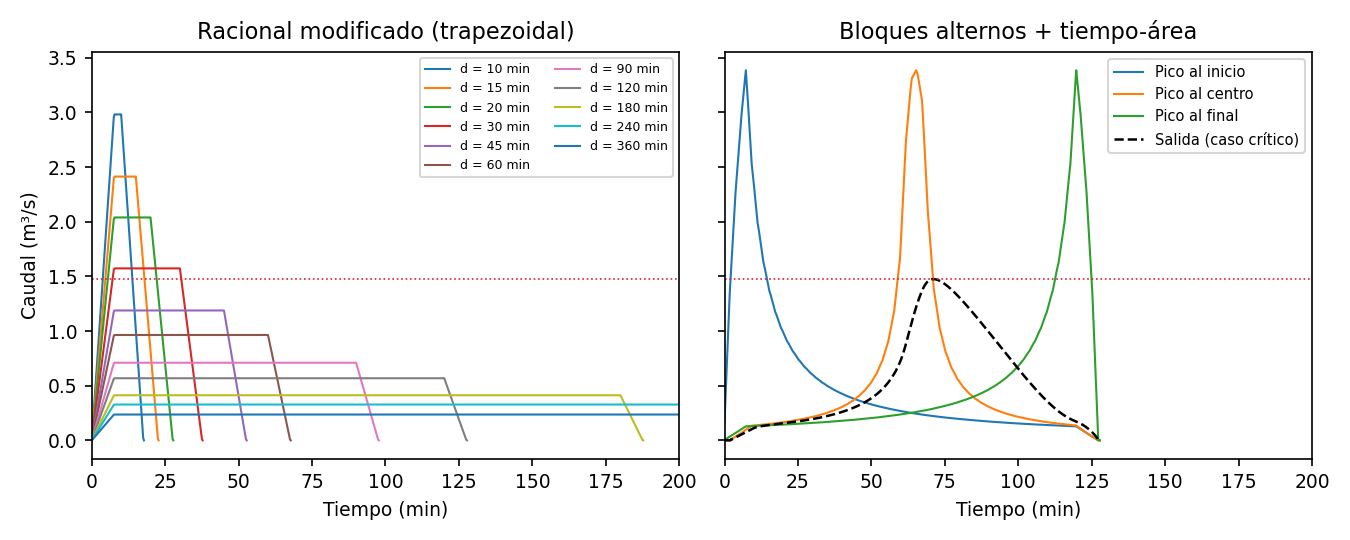
\includegraphics[width=0.95\linewidth]{hidrogramas_tanque_2_4B.png}
\nota{Línea punteada roja: caudal previo a la urbanización. Hietograma de 120 min en bloques de 2 min.}
\end{figure}

\begin{table}[H]
\caption{Volumen requerido por escenario}
\label{tab:tanque}
\centering\footnotesize
\begin{tabular}{llrrr}
\toprule
Método & Escenario & $Q_{\max}$ entrada (m$^3$/s) & Vol. entrada (m$^3$) & Vol. requerido (m$^3$) \\
\midrule
\csname @@input\endcsname ../../productos/punto2/final/tablas_tex/tanque.tex 
\bottomrule
\end{tabular}
\nota{Solo se listan las duraciones trapezoidales cuyo pico supera $Q_{pre}$; para las demás el volumen requerido es despreciable.}
\end{table}

\textbf{Duración crítica y volumen.} Con los hidrogramas trapezoidales del racional modificado, la duración crítica es \TrapCrit\ y exige \VolTrap\ m$^3$: las duraciones más cortas tienen un pico mayor pero poco volumen, y las más largas tienen un pico menor que $Q_{pre}$. El hietograma de bloques alternos exige más: \VolInicio, \VolCentro\ y \VolFinal\ m$^3$ con el pico al inicio, al centro y al final (tabla~\ref{tab:tanque}). Exige más porque concentra en una sola tormenta las intensidades de todas las duraciones con el mismo $T$, mientras que cada trapecio usa una intensidad constante. La posición del pico cambia el volumen: con el pico al inicio el tanque recibe lo más intenso cuando está vacío y descarga durante el resto de la tormenta; con el pico en el centro o al final llega cuando el tanque ya almacena el agua de la primera parte. El caso crítico es \EscCrit.

\textbf{Diseño.} Se recomienda un tanque de \LadoTanque\ $\times$ \LadoTanque\ m en planta, \Hutil\ m de profundidad útil y 0,5 m de borde libre (\VolUtil\ m$^3$ útiles), con un orificio de \DOrif\ m. En los 14 hidrogramas probados la salida máxima es \QsalMax\ m$^3$/s, sin superar $Q_{pre}$ (figura~\ref{fig:tanque}).

\subsection{Síntesis del punto 2}

Se escogió la lluvia de \Tdis\ años de duración igual al $t_c$ del SCS (\Idis\ mm/h), porque la obra es una alcantarilla de vía rural con consecuencias de falla moderadas. La mayor incertidumbre viene del tiempo de concentración, seguida de la IDF (es decir, de tener solo \NAnios\ años) y de $C$; la elección de la distribución pesa menos a esta duración. El riesgo real es mayor que el nominal: con el diámetro comercial mínimo el periodo de retorno efectivo cae a unos \Teff\ años, y por eso se recomienda \Drec\ m. Si la cuenca se urbaniza, el caudal casi se duplica y el tanque de \VolUtil\ m$^3$ lo devuelve al nivel previo. Si el clima intensifica las tormentas cortas a razón de un 7\,\% por grado \parencite{westra2014}, el riesgo efectivo aumentaría y el diseño debería revisarse.

% ================================================================== 4
\section{Conclusiones}

La demanda evaporativa de la cuenca Racarumi está controlada por la radiación, no por la temperatura ni por el viento; por eso los métodos radiativos la reproducen y los térmicos fallan, y por eso un método solo térmico exageraría la respuesta al calentamiento. La cuenca devuelve a la atmósfera algo más de la mitad de su lluvia, pero esa cifra es tan incierta como la lluvia misma: la diferencia entre productos de precipitación es la principal fuente de incertidumbre del balance. El régimen es estacional: la energía limita la evapotranspiración en la temporada húmeda y el agua en la seca, cuando la cuenca vive de la humedad acumulada en el suelo y, probablemente, del agua trasvasada. La demanda ha crecido, empujada por el calentamiento y por más radiación.

En el diseño, la principal lección es que el riesgo nominal subestima el real cuando la carga es incierta: en una microcuenca de minutos, la incertidumbre del tiempo de concentración y la de la IDF definen el tamaño de la obra más que la elección de la distribución. Un evento extremo en un registro de 20 años puede duplicar los cuantiles de duraciones largas respecto a una referencia regional, de modo que la comparación con KOSTRA es una verificación indispensable. Los límites principales son la cobertura espacial incompleta de ERA5-Land, la falta de datos de trasvases y de incertidumbre del caudal en el punto 1, y la salida sintética de la microcuenca y la longitud de 20 años del registro en el punto 2.

% ================================================================== 5
\section{Uso de inteligencia artificial}

Se aplicó el nivel A (abierto) de la política de IA del curso.

\begin{enumerate}
\item \textbf{Herramientas.} Codex/GPT de OpenAI (versión no registrada) en el desarrollo de los scripts; Claude Opus 5.5 de Anthropic, mediante Claude Code (noviembre de 2026), en la revisión final, la reorganización del repositorio y la redacción de este informe. \PENDIENTE{confirmar versiones y otras herramientas usadas}
\item \textbf{Tareas.} Escritura y depuración de scripts de descarga, procesamiento, ajuste de distribuciones, IDF, Monte Carlo y tránsito; organización de carpetas; revisión de coherencia entre cifras; borradores de redacción. En la revisión final, la IA rehízo el análisis del punto 2 en un único script, extrajo las cifras del punto 1 de las tablas existentes y redactó el informe.
\item \textbf{Verificación.} Se verificaron a mano la ETo FAO-56, Thornthwaite y Hargreaves en un día y una celda; Hargreaves contra \texttt{pyet}; la reproducción exacta de las tablas del apartado 1.3; el SHA-256 del raster de cobertura; la lectura de KOSTRA contra el valor publicado en la celda; y los diámetros y caudales de Manning con el cálculo directo.
\item \textbf{Propuestas corregidas o rechazadas.} En la revisión final se corrigieron: la fórmula del retardo del SCS, que tenía intercambiadas la pendiente y la retención; la omisión de la corrección de Weiss; un archivo de L-momentos con valores erróneos; el uso del bootstrap con ajustes de máxima verosimilitud degenerados; el diseño anterior del tanque, que no limitaba la salida al caudal previo a la urbanización; y la regla del diámetro, que no redondeaba al comercial superior. También se rechazó presentar el evento de 2021 como evidencia de cambio climático.
\item \textbf{Contribución de cada integrante.} \PENDIENTE{describir qué hizo cada integrante: Andrés Francisco Idrobo Hidrobo, Enmaly Aleli Manturano Grajeda y Jeyson Cristian Javier Irpanoca}
\end{enumerate}

El registro detallado de los cambios de la revisión final está en \texttt{anexos/registro\_revision\_final.md}.

% ================================================================== referencias
\newpage
\section*{Referencias}
\addcontentsline{toc}{section}{Referencias}
\begingroup
\setlength{\parindent}{-1.27cm}\setlength{\leftskip}{1.27cm}\setlength{\parskip}{6pt}\raggedright
\newcommand{\refx}[2]{\par\noindent\hspace*{-1.27cm}\hypertarget{#1}{}#2}

\refx{abatzoglou2018}{Abatzoglou, J. T., Dobrowski, S. Z., Parks, S. A. y Hegewisch, K. C. (2018). TerraClimate, a high-resolution global dataset of monthly climate and climatic water balance from 1958--2015. \textit{Scientific Data, 5}, Artículo 170191. https://doi.org/10.1038/sdata.2017.191}

\refx{allen1998}{Allen, R. G., Pereira, L. S., Raes, D. y Smith, M. (1998). \textit{Crop evapotranspiration: Guidelines for computing crop water requirements} (FAO Irrigation and Drainage Paper 56). FAO. https://www.fao.org/4/x0490e/x0490e00.htm}

\refx{bouchet1963}{Bouchet, R. J. (1963). Évapotranspiration réelle et potentielle, signification climatique. \textit{IAHS Publication, 62}, 134--142.}

\refx{brutsaert1998}{Brutsaert, W. y Parlange, M. B. (1998). Hydrologic cycle explains the evaporation paradox. \textit{Nature, 396}(6706), 30. https://doi.org/10.1038/23845}

\refx{budyko1974}{Budyko, M. I. (1974). \textit{Climate and life}. Academic Press.}

\refx{chow1988}{Chow, V. T., Maidment, D. R. y Mays, L. W. (1988). \textit{Applied hydrology}. McGraw-Hill.}

\refx{coles2001}{Coles, S. (2001). \textit{An introduction to statistical modeling of extreme values}. Springer. https://doi.org/10.1007/978-1-4471-3675-0}

\refx{debruin1987}{de Bruin, H. A. R. (1987). From Penman to Makkink. En J. C. Hooghart (Ed.), \textit{Evaporation and weather} (Proceedings and Information No.~39, pp.~5--31). TNO Committee on Hydrological Research.}

\refx{dejong2005}{de Jong, C., Collins, D. y Ranzi, R. (Eds.). (2005). \textit{Climate and hydrology in mountain areas}. Wiley. https://doi.org/10.1002/0470858249}

\refx{dwd2022}{Deutscher Wetterdienst. (2022). \textit{KOSTRA-DWD-2020: Starkniederschlagshöhen für Deutschland} [Conjunto de datos]. https://doi.org/10.5676/DWD/KOSTRA-DWD-2020}

\refx{dwd2026}{Deutscher Wetterdienst. (2026). \textit{Historische 10-minütige Niederschlagsdaten, Station 00020 Abtsgmünd-Untergröningen} [Conjunto de datos]. Climate Data Center. https://opendata.dwd.de/climate\_environment/CDC/}

\refx{dingman2015}{Dingman, S. L. (2015). \textit{Physical hydrology} (3.\textsuperscript{a} ed.). Waveland Press.}

\refx{fu1981}{Fu, B. P. (1981). On the calculation of the evaporation from land surface. \textit{Scientia Atmospherica Sinica, 5}(1), 23--31.}

\refx{gringorten1963}{Gringorten, I. I. (1963). A plotting rule for extreme probability paper. \textit{Journal of Geophysical Research, 68}(3), 813--814. https://doi.org/10.1029/JZ068i003p00813}

\refx{hosking1997}{Hosking, J. R. M. y Wallis, J. R. (1997). \textit{Regional frequency analysis: An approach based on L-moments}. Cambridge University Press. https://doi.org/10.1017/CBO9780511529443}

\refx{hoyos2026}{Hoyos, C. D. (2026). \textit{Evapotranspiración: el agua que vuelve al cielo} [Notas del curso de Hidrología]. Universidad Nacional de Colombia. https://carlosdhoyos.github.io/cursos/hidrologia/evapotranspiracion.html}

\refx{koutsoyiannis1998}{Koutsoyiannis, D., Kozonis, D. y Manetas, A. (1998). A mathematical framework for studying rainfall intensity-duration-frequency relationships. \textit{Journal of Hydrology, 206}(1--2), 118--135. https://doi.org/10.1016/S0022-1694(98)00097-3}

\refx{kuiry2021}{Kuiry, S. N. y Sen, D. (2021). \textit{Modelling hydrology, hydraulics and contaminant transport systems in Python}. CRC Press. https://doi.org/10.1201/9780429288579}

\refx{makkink1957}{Makkink, G. F. (1957). Testing the Penman formula by means of lysimeters. \textit{Journal of the Institution of Water Engineers, 11}, 277--288.}

\refx{martins2000}{Martins, E. S. y Stedinger, J. R. (2000). Generalized maximum-likelihood generalized extreme-value quantile estimators for hydrologic data. \textit{Water Resources Research, 36}(3), 737--744. https://doi.org/10.1029/1999WR900330}

\refx{mcvicar2012}{McVicar, T. R., Roderick, M. L., Donohue, R. J., Li, L. T., Van Niel, T. G., Thomas, A., Grieser, J., Jhajharia, D., Himri, Y., Mahowald, N. M., Mescherskaya, A. V., Kruger, A. C., Rehman, S. y Dinpashoh, Y. (2012). Global review and synthesis of trends in observed terrestrial near-surface wind speeds: Implications for evaporation. \textit{Journal of Hydrology, 416--417}, 182--205. https://doi.org/10.1016/j.jhydrol.2011.10.024}

\refx{milly2016}{Milly, P. C. D. y Dunne, K. A. (2016). Potential evapotranspiration and continental drying. \textit{Nature Climate Change, 6}(10), 946--949. https://doi.org/10.1038/nclimate3046}

\refx{miralles2011}{Miralles, D. G., Holmes, T. R. H., De Jeu, R. A. M., Gash, J. H., Meesters, A. G. C. A. y Dolman, A. J. (2011). Global land-surface evaporation estimated from satellite-based observations. \textit{Hydrology and Earth System Sciences, 15}(2), 453--469. https://doi.org/10.5194/hess-15-453-2011}

\refx{mu2011}{Mu, Q., Zhao, M. y Running, S. W. (2011). Improvements to a MODIS global terrestrial evapotranspiration algorithm. \textit{Remote Sensing of Environment, 115}(8), 1781--1800. https://doi.org/10.1016/j.rse.2011.02.019}

\refx{munozsabater2021}{Muñoz-Sabater, J., Dutra, E., Agustí-Panareda, A., Albergel, C., Arduini, G., Balsamo, G., Boussetta, S., Choulga, M., Harrigan, S., Hersbach, H., Martens, B., Miralles, D. G., Piles, M., Rodríguez-Fernández, N. J., Zsoter, E., Buontempo, C. y Thépaut, J.-N. (2021). ERA5-Land: A state-of-the-art global reanalysis dataset for land applications. \textit{Earth System Science Data, 13}(9), 4349--4383. https://doi.org/10.5194/essd-13-4349-2021}

\refx{nrcs2010}{Natural Resources Conservation Service. (2010). Time of concentration. En \textit{National engineering handbook, part 630 hydrology} (cap. 15). U.S. Department of Agriculture.}

\refx{pastorello2020}{Pastorello, G., Trotta, C., Canfora, E., Chu, H., Christianson, D., Cheah, Y.-W., Poindexter, C., Chen, J., Elbashandy, A., Humphrey, M., Isaac, P., Polidori, D., Reichstein, M., Ribeca, A., van Ingen, C., Vuichard, N., Zhang, L., Amiro, B., Ammann, C., \ldots Papale, D. (2020). The FLUXNET2015 dataset and the ONEFlux processing pipeline for eddy covariance data. \textit{Scientific Data, 7}, Artículo 225. https://doi.org/10.1038/s41597-020-0534-3}

\refx{roderick2002}{Roderick, M. L. y Farquhar, G. D. (2002). The cause of decreased pan evaporation over the past 50 years. \textit{Science, 298}(5597), 1410--1411. https://doi.org/10.1126/science.1075390-a}

\refx{sankarasubramanian2001}{Sankarasubramanian, A., Vogel, R. M. y Limbrunner, J. F. (2001). Climate elasticity of streamflow in the United States. \textit{Water Resources Research, 37}(6), 1771--1781. https://doi.org/10.1029/2000WR900330}

\refx{shaw2010}{Shaw, E. M., Beven, K. J., Chappell, N. A. y Lamb, R. (2010). \textit{Hydrology in practice} (4.\textsuperscript{a} ed.). Spon Press.}

\refx{svensson2010}{Svensson, C. y Jones, D. A. (2010). Review of methods for deriving areal reduction factors. \textit{Journal of Flood Risk Management, 3}(3), 232--245. https://doi.org/10.1111/j.1753-318X.2010.01075.x}

\refx{usgs2013}{U.S. Geological Survey. (2013). \textit{Shuttle Radar Topography Mission 1 arc-second global} [Conjunto de datos]. https://doi.org/10.5066/F7PR7TFT}

\refx{weiss1964}{Weiss, L. L. (1964). Ratio of true to fixed-interval maximum rainfall. \textit{Journal of the Hydraulics Division, 90}(HY1), 77--82. https://doi.org/10.1061/JYCEAJ.0001008}

\refx{westra2014}{Westra, S., Fowler, H. J., Evans, J. P., Alexander, L. V., Berg, P., Johnson, F., Kendon, E. J., Lenderink, G. y Roberts, N. M. (2014). Future changes to the intensity and frequency of short-duration extreme rainfall. \textit{Reviews of Geophysics, 52}(3), 522--555. https://doi.org/10.1002/2014RG000464}

\refx{zanaga2022}{Zanaga, D., Van De Kerchove, R., Daems, D., De Keersmaecker, W., Brockmann, C., Kirches, G., Wevers, J., Cartus, O., Santoro, M., Fritz, S., Lesiv, M., Herold, M., Tsendbazar, N.-E., Xu, P., Ramoino, F. y Arino, O. (2022). \textit{ESA WorldCover 10 m 2021 v200} [Conjunto de datos]. Zenodo. https://doi.org/10.5281/zenodo.7254221}
\par\endgroup

\end{document}
